\section{Results} 
We consider an animal who interacts with an environment over a sequence of states, actions and rewards. Their reward learning is embedded in the now standard Markov decision process. It's goal is to select actions in a way that maximizes the total reward collected from the environment for every state $\mathbf{S}$ (Eq \ref{eq:V_R}).

\begin{equation}
	\label{eq:V_R}
	V_R(\mathbf{S}) = \argmax_{\mathbf{A}} \Big [ \sum_T R \Big ]
\end{equation}

How should an animal do this? To maximize reward an animal must tradeoff between exploration, and exploitation. The standard way of approaching this tradeoff is to assume, ``The agent must try a variety of actions and progressively favor those that appear to be best'' \cite{Sutton2018}. Here we suggest two fairly radical changes to this standard formula. Don’t stop searching progressively, do so suddenly (greedily). Explore only for learnings sake, out of curiosity \citep{Kidd2015}. To demonstrate the advantages of this first we need to establish some shared formalities.

\subsubsection{Markovian formalities}
Our Markov decision process (MDP) consists of states of real valued vectors $\mathbf{S}$ from a finite set $\mathcal{S}$ of size $n$. As are actions, $\mathbf{A}$ from a finite set $\mathcal{A}$ of size $k$. Rewards are non-negative real numbers, $R$. Transitions from state to state are handled by the transition function $\Lambda(\mathbf{S})$. In our mathmatics we assume $\Lambda$ is a deterministic function of its inputs. In our simulations we assume it is a stochastic function.

To study learning, memory and curiosity hollistically we assume animals can ``fuse'' the elements of the MDP into single observations, $\mathbf{X}$.  It is convenient to assume there observations are embedded in a finite real space, $\mathbf{X} \in \mathcal{X}$ of size $l$. This fusing is imagined to happen via a communication channel, $T$, which is identical to out observation function, $T(\mathbf{S},\mathbf{A},\mathbf{S'},R,\mathbf{M})$. $\mathbf{M}$ is the animal's memory, that we define below. 

Observations made by $T$ can be internally generated from memory $\mathbf{M}$, or externally generated from the environment ($\mathbf{S}$,$\mathbf{S'}$). Or both in combination, as happens in recurrent neural circuits. Observations may contain action information $\mathbf{A}$ but this optional. Observations may contain reward information $R$ or not. Though ommiting reward would hamper solving dilemma.

\subsection{A general kind of curiosity} 
To make our eventual solution general, we first need to separate reward value from information value in a principled and general way. We do this axiomatically. Working models of curiosity tend to conflate the learning rule, with the objective itself. We will now describe an optimal value, but deterministic model, of curiosity. It is defined by some easily satisfiable requirements (axioms). This basis makes curiosity domain general, and learning rule independent. We assume curiosity is value driven, and should be as time-efficient as possible.

We reason that the value of any observation $\mathbf{X}$ made by an animal depends entirely on what an animal learns by making that observation–-how it changes an animal's memory. But how can we define memory in a way that is general, but practically useful?

Sustained firing, the strength between two synapses, elevated Calcium concentration are three simple examples of learning and memory in the nervous system. Each of these examples though can be represented as a vector space. In fact, most any memory system can be so defined. 


\subsubsection{Memory formalities}
We define memory as a set of real valued numbers, embedded in a finite space that is closed and bounded with $p$ dimensions. In practice we regard memory $\mathbf{M}$ as learning something about a sequence of observations ($\mathbf{X}_0$ $\mathbf{X}_1$, $\mathbf{X}_2$, ...) which have arrived via a the communications channel $T$. 

A learning function is then any function $f$ that maps observations $\mathbf{X}$ into memory $\mathbf{M}$. This $f$ is considered to be a valid learning function as long as the mapping changes $\mathbf{M}$ some small amount. A non-constant mapping, in other words. Using recursive notation, this kind of learning is denoted by $\mathbf{M} \leftarrow f(\mathbf{X},\mathbf{M}) $. Though we will sometimes use $\mathbf{M'}$ to denote the updated memory. Other times we will add subscripts, like $\mathbf{X}_0,\mathbf{X}_1,ldots$, to express the history of a memory, or the path is has followed. 

We can also define a forgetting function that \textit{can be any function} that inverts the memory, $f^{-1}(\mathbf{X};\ \mathbf{M}') \rightarrow \mathbf{M}$. Forgetting might not seem crucial, here. But it will prove essential later on in developing exploration algorithms that provably maximize $\hat E$. 

For individual animals we assume $f$ and $f^{-1}$ have been chosen by evolution and experience to be suitable and efficient for the environment \cite{Valiant1984,Thrun1992a,Schmidhuber1991,Oudeyer2016,Pathak2017,Gottlieb2018,Wilson2020,Schwartenbeck2019}. 


\subsubsection{Axiomatic information value} 
Our definition of information value closely follows that of Shannon and his definition of a communication channel. If the communication channel is agnostic to semantic considerations, as in Shannon's definition, we reason its information value should be agnostic as well.

If we have a memory $\mathbf{M}$, which has been learned by $f$ over a history of observations, $(\mathbf{X_0},\mathbf{X_1},...)$, Can we measure how much value the next observation $\mathbf{X_t}$ should have? We think this measure $\hat E$ should have certain intuitive properties.

\\
\\
\noindent
\textbf{Axiom 1} (Axiom of Memory). $\hat E$ depends only on difference $\delta \mathbf{M}$ between $\mathbf{M}$ and $\mathbf{M'}$.

That is, the value of an observation $\mathbf{X|$} depends only on how
the current memory changes. 
\\
\noindent
\textbf{Axiom 2} (Axiom of Change).  $\hat E = 0$ if and only if $\delta M = 0$. 

That is, an observation that doesn’t change the memory has no value.
\\
\noindent
\textbf{Axiom 3} (Axiom of Scholarship). $\hat E \ge 0$.

That is, all (new) information is in principle valuable even its consequences are later found to be negative.
\\
\noindent
\textbf{Axiom 4} (Axiom of Completeness) $\hat E$ should increase monotonically with the total change in memory. 

That is, there should be a one-to-one relationship how memory changes and how information is valued.
\\
\noindent
\textbf{Axiom 4} (Axiom of Equilibrium) For the same observation $\hat E$ should approach 0 in finite time.

That is, learning on $\mathbf{M}$ makes continual progress toward equilibrium (i.e. self-consistency) with each observation, after a finite time period has passed. After this it will approach a steady-state value of $\delta \mathbf{M} \rightarrow 0$ and $\hat E \rightarrow 0$.

All we have really done in these axioms is remove any mention of a learning rule, its properties, or learning target, its propertiess \cite{Itti2009,Jaegle2019,Schmidhuber1991,Inglis2001,Reddy2016,Pirolli2007}. This is important not for its own sake but because, we it lets use consider information value independent of any semantics. Anything we prove in this general setting will be therefore be true for any learning algorithm, who meets our requirements. 

\subsubsection{Practical (geometric) information value}
Meeting our requirements is not difficult. The practical example of axiomatic value we use throughout this paper is based on the geometric norm. Though not necessaailry a unique solution this is quite a natural way, based only the dynamics and ``shape'' of the memory space itself (Eq \ref{eq:E_norm}). 

\begin{equation}
	\label{eq:E_norm}
	\hat E = || \ f(\mathbf{M},\mathbf{X}) - \mathbf{M} \ ||
\end{equation}

To ensure equilibrium in Eq \ref{eq:E_norm}, we require $\nabla^2 \mathbf{M} < 0$ for all $ t \ge T^*$. Informally, the idea here is that any notion of sensible and useful learning must in time converge, which we take to mean that in finite time $\hat E$ must approach 0 (Fig.~\ref{fig:cartoon}). We term this consistent learning.

% TODO - update X on plot to match new text notation
\begin{figure}
	\begin{fullwidth}
	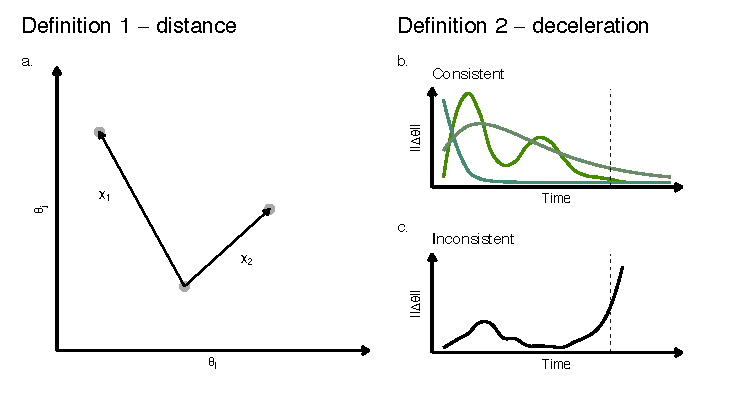
\includegraphics[width=0.7\linewidth]{img/cartoon.pdf} 
	\caption{Geometric information value, and our constraints on its dynamics. 
	\textbf{a}. This panel illustrates a two dimensional memory. The information value of two observations $\mathbf{X}_1$ and $\mathbf{X}_2$ depends on the norm of memory with learning. Here we show this distance as a euclidean norm, denoted as a black arrow.
	\textbf{b-c} This panel illustrates learning dynamics with time (over a series of observations that are not shown). If information value becomes decelerating in finite time bound, then we say that learning is consistent with Def. 2. This is shown in panel b. The bound is depicted as a dotted line. If learning does not decelerate, then it is said to be inconsistent (Panel c). \textit{It is important to note:} our account of information value and curiosity does not work when learning is inconsistent.
  	}
	\label{fig:cartoon} 
	% \figsupp{} % No limit on these.
	\end{fullwidth}
\end{figure}

% TODO - HERE
% Mention we don't need to carry an exact complete history, as POMPDS do in info space does.
\subsubsection{Deterministic curiosity}
A nice solution to maximizing $\hat E$, and so ideal curiosity, would be a Bellman solution \citep{Bellmann1954} because it guarantees optimal value using just recursion, a very biological idea. It is convenient also because the Bellman equation is the basis for the theory of reinforcement learning \citep{Sutton2018}. 

The common way to arrive at Bellman solution is to assume a Markov decision space. This is problem for memory because it naturally has a long-term path dependence, which breaks the Markov assumption and its neeeded claim of optimal substructure. To get around this we prove that forgetting is another way to achieve optimal substructure. 

Given an arbitrary starting value $E_0 > 0$, the best solution to maximizing $\hat E$ is given by Eq.~\ref{eq:V_E_bellman}. A full derivation for this fact is provided in the Appendix. 

\begin{equation}
	\label{eq:V_E_bellman} 
	V^{\pi_{E}}(\mathbf{X}_0) = \argmax_{\mathbf{A}} \Big [ E_0 + V_E(\mathbf{X}_1) \Big ]
\end{equation}

As long learning about the different observations $\mathbf{X}$ is independent, and as long as learning continues until steady-state, defined as $E_t < \eta$, there are many equally good solutions. Under these conditions we can simplify Eq. \ref{eq:V_E_bellman} further, giving Eq. \ref{eq:EE}. 

\begin{equation}
	\label{eq:EE} 
	V^{\pi_{E}}(\mathbf{X}_0)  \approxeq \argmax_{\mathbf{A}} \Big [ E_0 + E_1 \Big ]
	% V^{\pi}_E(\mathbf{X}_0) = \argmax_{\mathbf{A}} \Big [ E_0 + E(f(\mathbf{X}_0,\mathbf{M}),\mathbf{M}) \Big ]
\end{equation}

\subsection{A note on exploration quality}
Having a policy $\pi_E^*$ that maximizes $\hat E$ does not necessarily ensure that exploration is of good quality. We think it is reasonable to call an exploration good if it meets the three criteria below. In Theorem~\ref{needed} we prove that our Bellman solution $\pi_E$ satisfies these, when $\eta > 0$.

% TODO - add to appendix
% heorem 2. The optimal policy π∗E must visit each state in s ∈ S at least once.
% • Theorem 3. The optimal policy π∗E must revisit each s ∈ S until learning about each state s until the memory reaches equilibrium dM = 0.

\begin{enumerate}
	\item Exploration should visit all available states of the environment at least once.
	\item Exploration should cease when learning has plateaued.
	\item Exploration should take as few steps as possible to achieve 1 and 2.
\end{enumerate}


\subsection{A note on boredom}
The central failure mode of curiosity is what we'll call minutia, defined as those learning that has little to no use, ever. A good example of this is to, ``Imagine a scenario where the agent is observing the movement of tree leaves in a breeze. Since it is inherently hard to model breeze, it is even harder to predict the location of each leaf'' \cite{Pathak2017}. This will imply, they note, a curious agent will always remain curious about chaos in the leaves even though they have no hope of successful learning of them.

To limit curiosity we will use boredom which we consider an adaptive trait. Others have considered boredom constructilvy arguing it is a useful way to motivate aversive tasks \citep{Bench2013}, or curiosity \cite{Loewenstein1994}. We take a slightly different view. We treat boredom as a tunable free parameter, $\eta \ge 0$. We consider boredom as a means to ignore marginal value, by requiring curious exploration to stop once $E \le \eta$. 


\subsection{A win-stay, lose-switch solution}
How can we justify using curiosity for the dilemma when the goal of exploitation is reward collection? Curiousity is just as important for survival as reward collection \cite{Thrun1992}. Curiosity is a primary drive in most, if not all, animals \cite{Inglis2001}. It is as strong, if not sometimes stronger, than the drive for reward \cite{Loewenstein1994,Kidd2015,Gottlieb2018}. 

Still, intuition suggests that curiosity is wrong-headed. Searching in an open-ended way for information must be less efficient than a direct search for reward? In answer to this we make two conjectures.

\textbf{A hypothesis of equal important} (Conjecture 1): Reward value and information value are equally important.

If both reward and information are equally important, then time is not wasted in a curious search, and so the process is not \textit{necessarily} inefficient or even indirect. The question becomes instead, is curiosity practical enough to serve as a usseful trick to solve reward collection search problems? This leads us to the next conjecture. 

\textbf{The curiosity trick} (Conjecture 2): Curiosity is a sufficient solution to exploration (when learning is the goal)

It's worth noting here that curiosity, as an algorithm, is highly effective at solving optimization problems \cite{Schmidhuber1991,Pathak2017,Stanton2018,Lehman201,Mouret2011b1,Fister2019,Mouret2015,Colas2020,Cully2015,Pathak2017,Schwartenbeck2019.Laversanne-Finot2018}. 

If reward and information are equally important, how can an animal go about balancing them? If you accept our conjectures then answering this question is the same as answering the dilemma. To solve this dual value learning problem we’ve posed–-information and reward maximization–-we need an algorithm that can maximize the total value of both objectives. We found a simple answer in game theory and in the computer science sub-field of optimal scheduling.

Win-stay lose-shift is a strategy famous from game theory \citep{Nowak1993}, where a player will keep its current strategy under winning conditions, and shift otherwise. We see the same kind of patterning as useful here, except the ``players'' are two different policies inside the animal. They are competing for behavioral control. Imagine that in the previous action our bee from Fig. ~\ref{fig:bee} observed 0.7 units of information value, $\hat E$, and no reward (i.e. 0). Using our rule on the next action, the bee should then choose its exploration policy. Let us say that this time $\hat E$ decreases to 0.6, and a reward value of 1.0 is observed. Now the bee should change its strategy for the next round, to exploit instead. In general then if there was more reward value then information value last round ($R_{t-1} > E_{t-1}$), our rule dictates an animal should choose the reward policy. If information value dominated, $E_{t-1} > \ge R_{t-1}$, then it should choose the information gathering policy.

Here we propose that a win-stay, lose-switch strategy is in fact an optimal and tractable solution to the scheduling problem of exploration (by curiosity) and exploitation (for reward).

To prove the optimality of our rule we will use regret minimization, which is a standard metric of optimality in reinforcement learning \citep{Sutton2018}. Regret is a numerical quantity of the difference between the most valuable choice and the value of the choice that was made. To approximate regret $G$ we use Eq.~\ref{eq:regret}, where $V$ is the value of the chosen action, and $V^*$ is the maximum value. 

\begin{equation}
\label{eq:regret}
	G = V^* - V
\end{equation}

An optimal value algorithm always makes the most valuable choice. It therefore will have zero regret, by Eq.~\ref{eq:regret}. This is impossible to achieve, of course, using stochastic search. To find the algorithm that maximizes both information and reward value with zero regret, we therefore need a deterministic method. 

To prove things about our solution we will move from game theory, which gave us our inspiration, to the field of optimal scheduling \citep{Bellmann1954,Roughgarden2019}. Put another way, we will now answer the question, when does win-stay, lose-switch strategy work as an optimal scheduler? 

We imagine the policies for exploration and exploitation acting as two possible ``jobs'' competing for control of behavior, a fixed resource. We know by definition that each of these jobs produces non-negative values which an optimal job scheduler could use: $\hat E$ for information or $R$ for reward/reinforcement learning. We can also ensure, again by definition, that each of the jobs takes a constant amount of time and that each policy can only take one action at a time. These two properties, and one further assumption, are sufficient.

We believe it is also reasonable to assume that there will be no model of the environment available to the learner at the start of a problem, and that its environment is nonlinear but deterministic. 

We arrived at our solution by taking the simplest possible path available. We just wrote down the simplest equation that could have zero regret answer, and began to study that. This is Eq.~\ref{eq:meta_greedy}. We refer to it as a meta-greedy algorithm. It decides in greedy fashion which of our independent policies to use.

\begin{equation}
\label{eq:pipi} 
\Pi^{\pi} = \ \Big \{ \pi_E,\ \pi_R \Big \}
\end{equation}

\begin{equation}
\label{eq:meta_greedy} 
	\argmax_{\Pi^{\pi}} \ \Big [ \hat E - \eta,\ R \Big ]_{\textbf{(2, 1)}}
\end{equation}
	
In Eq \ref{eq:meta_greedy} we modified argmax notation to include a subscript vector to denote a ranking for which value/policy should be preferred in the event of a tie. In this case its $(2,1)$. We did this because an exact rule for tie breaking is it turns out critical. 

In Theorem \ref{theorem:meta_total} we prove Eq. \ref{eq:meta_greedy} is Bellman optimal, and so it will always find a maximum value sequence of $\hat E$ and $R$ values. Given, that is, that the environment is deterministic. 

% In Theorem \ref{theorem:meta} we also prove that with a judicious choice in boredom $\eta$, the reward policy $\pi_R$ will also converge to its optimal value, assuming that it has one. Full details for these proofs are found in the mathematical appendix.

In Eq \ref{eq:meta_greedy} we compare reward $R$ and information value $\het E$ but have not ensured they have same ``units'', or are comparible valuables. We sidestep this isssue by limiting the probability of having zero reward to be, itself, non-zero. That is, $p(R_t=0) > 0$. We also limit $E_0$, the first set of values, to be positive and non-zero when used with boredom, $(E_0 - \eta) \geq 0$. These constraints ensure complete ``good'' exploration (defined above) which in turn ensures optimal reward learning is possible.

\subsection{A note about subjective reward value}
We have been studying a kind of reinforcement learning where the value of a reward is fixed. That is, where environment reward value $R$ is always equal to it subjective value to the animal $\hat R$. It is the most common style of reinforcement learning \citep{Sutton2018}. In natural behavior though the motivational value of reward often declines as the animal reaches satiety. We'll call reward learning like this the homeostatic style \citep{Keramati2014,Juechems2019,Munch2020}. Fortunately, it has already been proven that a reward collection policy designed for one style will work for the other, at least this is so an infinite time-horizon \citep{Keramati2014}. However to use Eq. \ref{eq:meta_greedy} for reward homeostasis we need to make one modification. Under homeostasis ties between values in Eq. \ref{eq:meta_greedy} should be broken in favor of exploration, and information seeking. This modification leads to Eq. \ref{eq:meta_greedy_h}. This equation implies under reward homeostasis an animal's default policy is information seeking, and therefore environmental exploration.

\begin{equation}
	\label{eq:meta_greedy_h} 
	\argmax_{\Pi^{\pi}} \ \Big [ \hat E - \eta,\ \hat R \Big ]_{\textbf{(1, 2)}}
\end{equation}



\subsection{Information collection in practice}
The work so far has built up the idea that the most valuable, and most efficient, curious search will come from a deterministic algorithm. That is, every step strictly maximizes $\hat E$. It is this determinism which will let us resolve the dilemma, later on. A deterministic view of exploration seems at odds with how the problem is generally viewed today, which involves searching with some amount of randomness. Whereas if our analysis is correct, randomness is not needed or desirable, as it must lead to less value and a longer search. 

We confirm and illustrate this result using an example of a simple information foraging task (Task 1; Fig.\label{fig:task_outline1}). This variation of the bandit task \citep{Sutton2018} replaces rewards with information, in this case colors. On each selection, the agent sees one of two colors according to a specific probability shown in Fig. ~\ref{fig:payout}a. When the relative color probabilities are more similar that arm has more entropy and so more to learn and more information value. Arms that are certain to present only one color lose their informative value quickly.

The results of this simple information seeking task are shown in Figure~\ref{fig:curiosity1}. Deterministic curiosity in this task generated more information value, in less time, and with zero regret when compared against a stochastic agent using more directed random search. As our work here predicts, noise only made the search happen slower and lead to regret. Besides offering a concrete example, performance in Task 1 is a first step in showing that even though $\pi_E$'s optimality is proven for a deterministic environment, it can perform well in other settings.

\begin{figure}
	\begin{fullwidth}
	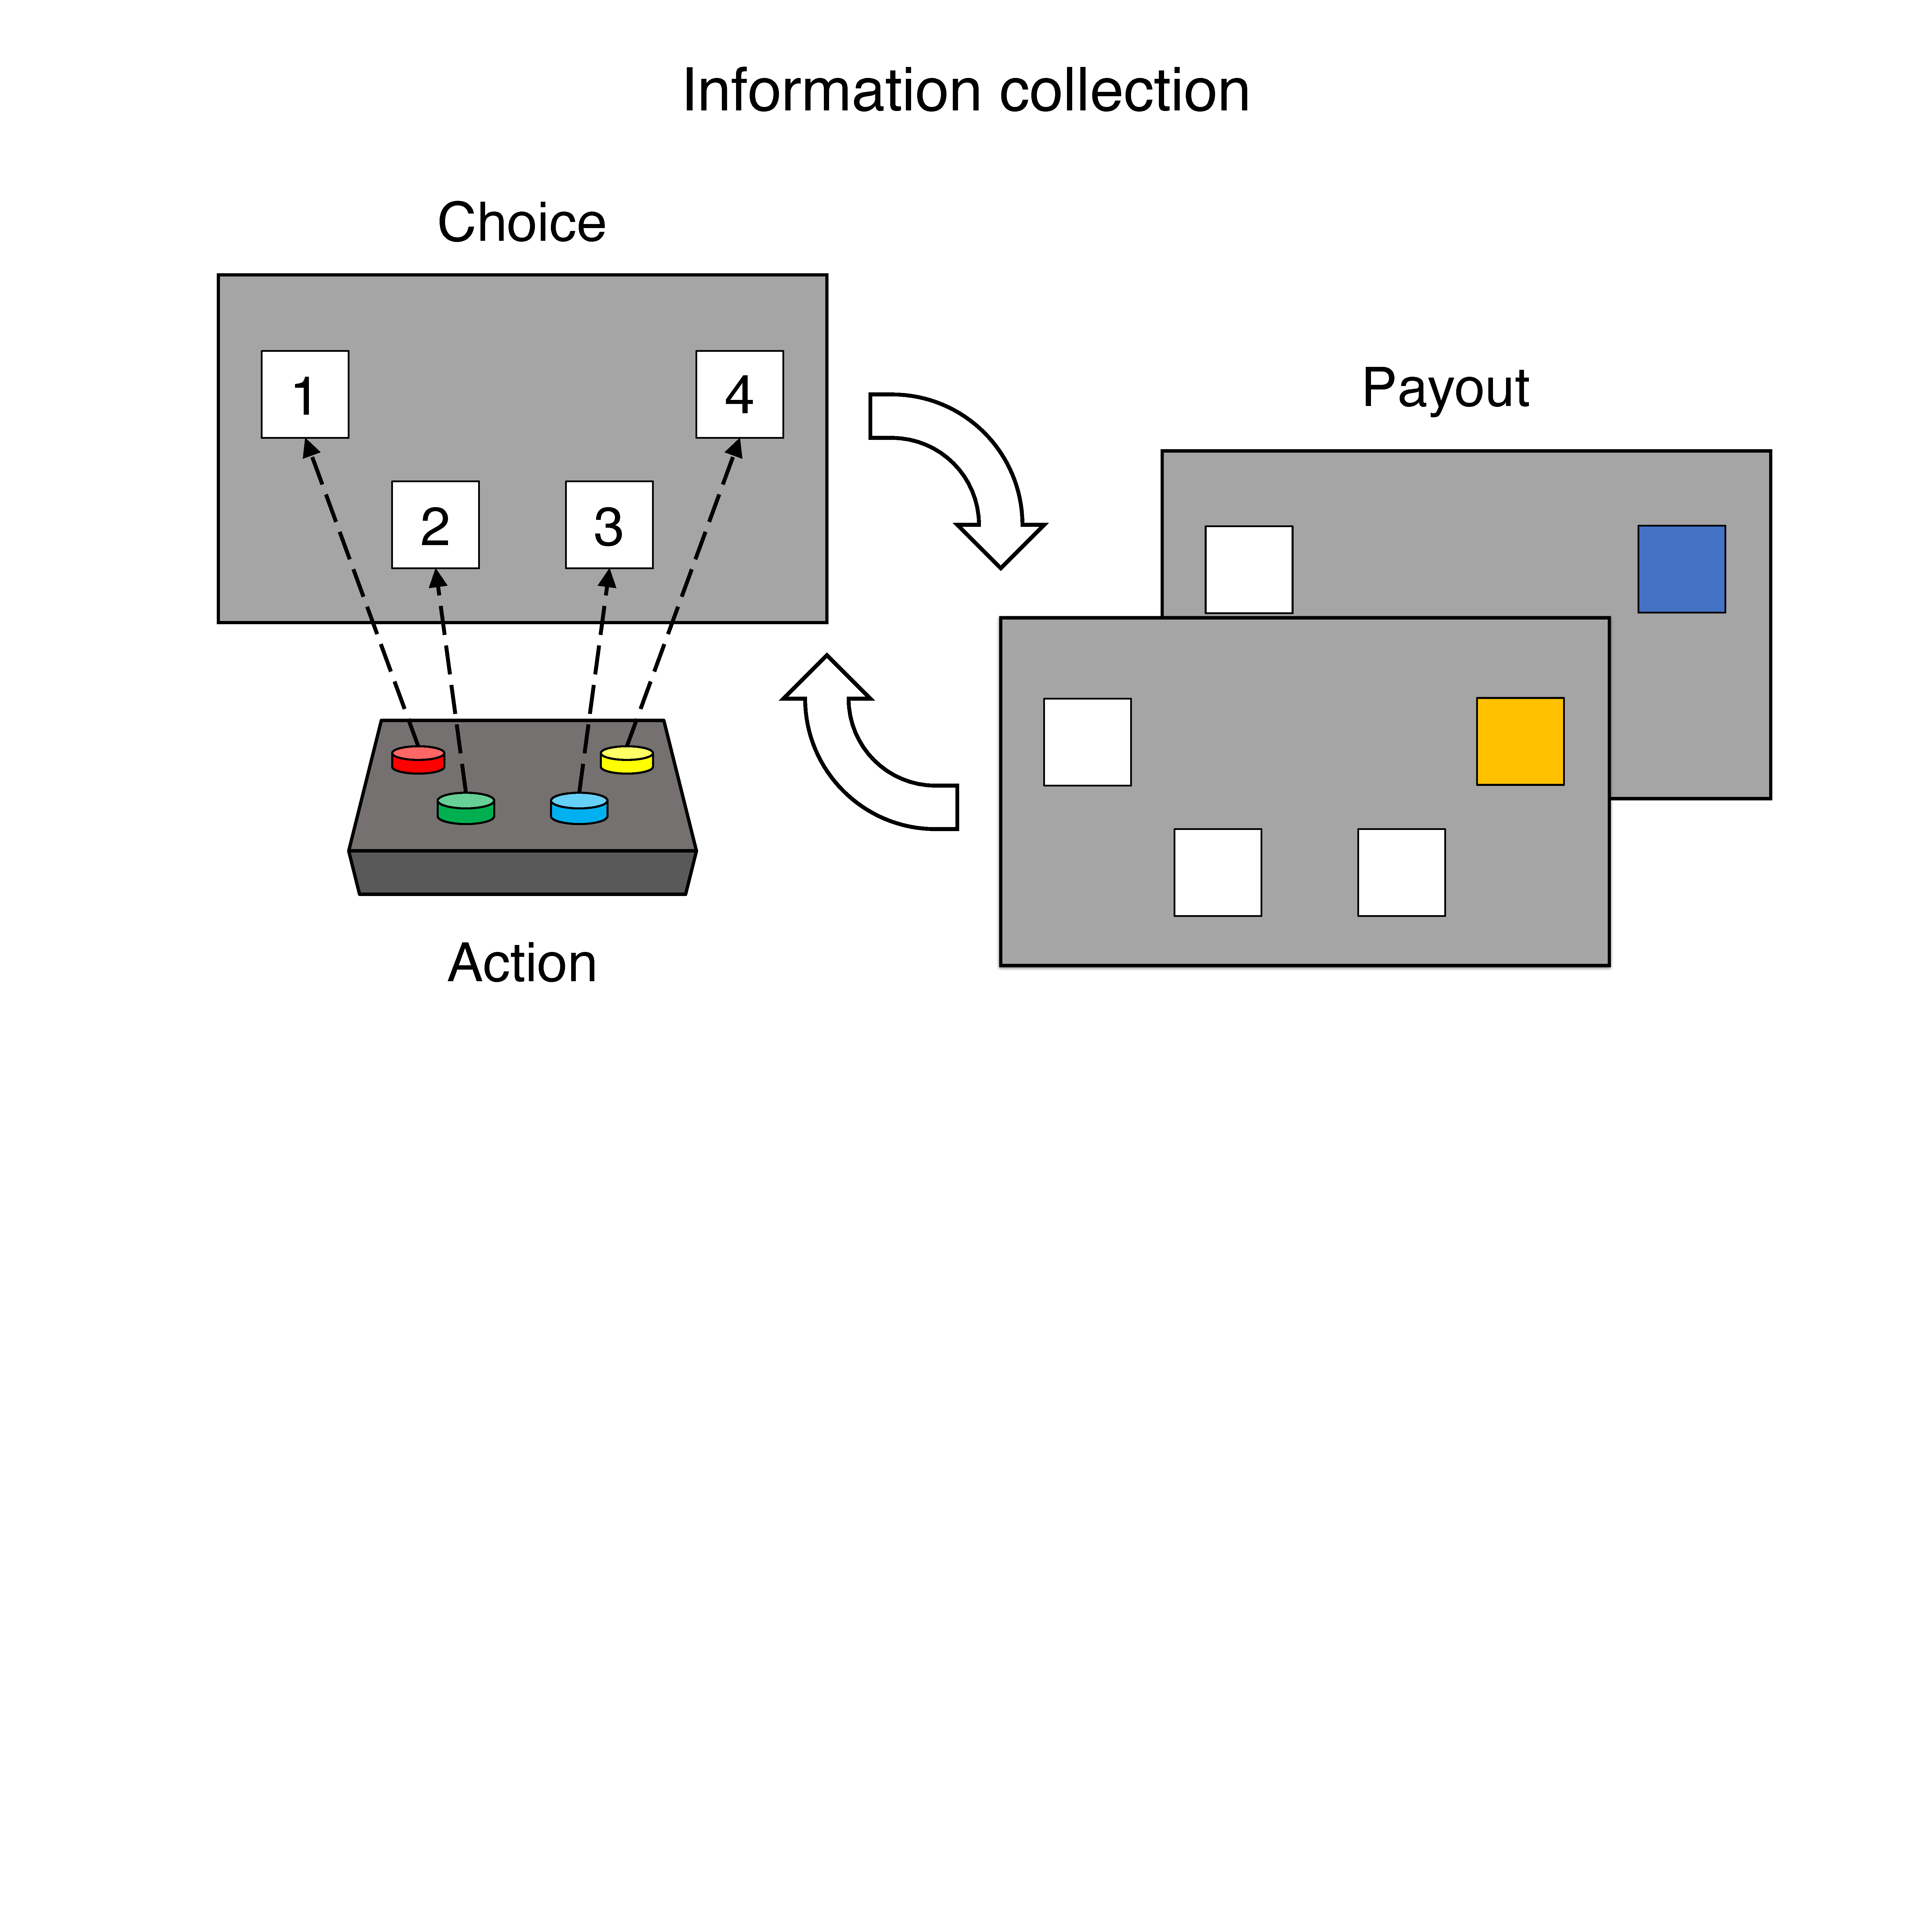
\includegraphics[width=.55\linewidth]{img/task_outline1.pdf} 
	\caption{A simple four choice information foraging task. The information in this task is a yellow or blue stimulus, which can change from trial to trial. A good learner in this task is one who tries to learn the probabilities of all the symbols in each of the four choices. The more random the stimuli are in a choice, the more potential information/entropy there is to learn. \textit{Note}: the information payout structure is shown below (Fig.~\ref{fig:payout}a}).
	\label{fig:task_outline1} 
	\end{fullwidth}
\end{figure}

\begin{figure}
	\begin{fullwidth}
	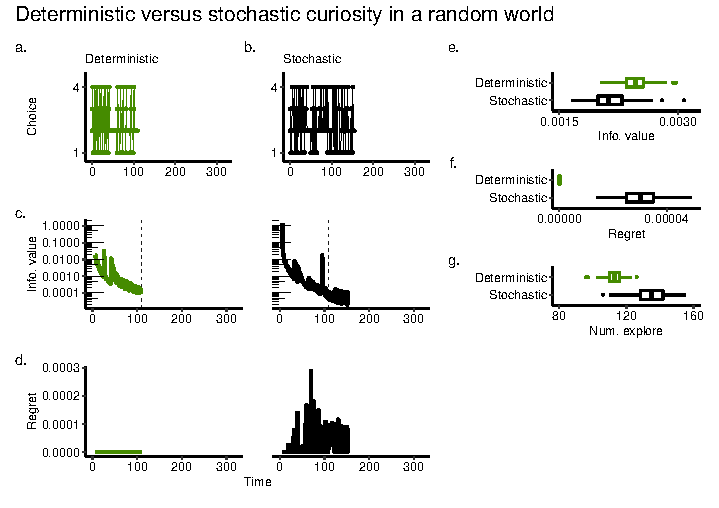
\includegraphics[width=.7\linewidth]{img/curiosity1.pdf} 
	\caption{Comparing deterministic versus stochastic variations of the same curiosity algorithm, in a simple information foraging task (Task 1). Deterministic results are shown in the left column, and stochastic are shown in the right. The hyperparameters for both models were found by random search, which is described in the Methods.
	\textbf{a-b}. Examples of choice behavior.
	\textbf{c-d}. Information value plotted with time for the behavior shown in a-b.
	\textbf{e-f}. Regret plotted with time for the behavior shown in a-b. Note how our only deterministic curiosity generates zero regret, inline with theoretical predictions.
	\textbf{e}. Average information value for 100 independent simulations. Large values mean a more efficient search.
	\textbf{f}. Average regret for 100 independent simulations. Ideal exploration should have no regret. 
	\textbf{g}. Number of steps it took to reach the boredom threshold $eta$. Smaller values imply a faster search.
	}
	\label{fig:curiosity1} 
	\end{fullwidth}
\end{figure}


\subsection{Reward collection in practice} 
Our approach does not mathematically ensure a dual value solution to the dilemma maximizes reward value comparerd with other well-established methods. To findout we meaasured total reward collected over 7 tasks and 10 agents, including ours. Each agent's parameters were independently optimized for each task. For a brief description of each agent, see Table~\ref{tab:agents}. They all have in common that their central goal is to maximize total reward value, though this is often supplemented by some other goal, an intrinic reward or bonus \cite{Ng1999,Sutton1998}. 

The general form of the 7 tasks are depicted in Fig~\ref{fig:task_outline2}. As with our first task (Fig. ~\ref{fig:task_outline1}) they are all variations of the classic multi-armed bandit \citep{Sutton2018}. The payouts for each of the tasks are shown separately in Fig.~\ref{fig:payout}. Each task was designed to either test exploration performance in a way that matches recent experimental studies, or to test the limits of curiosity. Every trial has a set of $n$ choices. Each choice returns a “payout”, according to a predetermined probability. Payouts are information, a reward, or both. Note that, as in Task 1, information was symbolic, denoted by a color code, “yellow” and “blue” and as is custom reward was a positive real number. 

The results in full for all tasks and exploration strategies are shown in Fig.~\ref{fig:summary}. All agents, including ours, used the same exploitation policy based on the temporal difference learning rule \citep{Sutton2018} (Methods).

\begin{figure}
	\begin{fullwidth}
	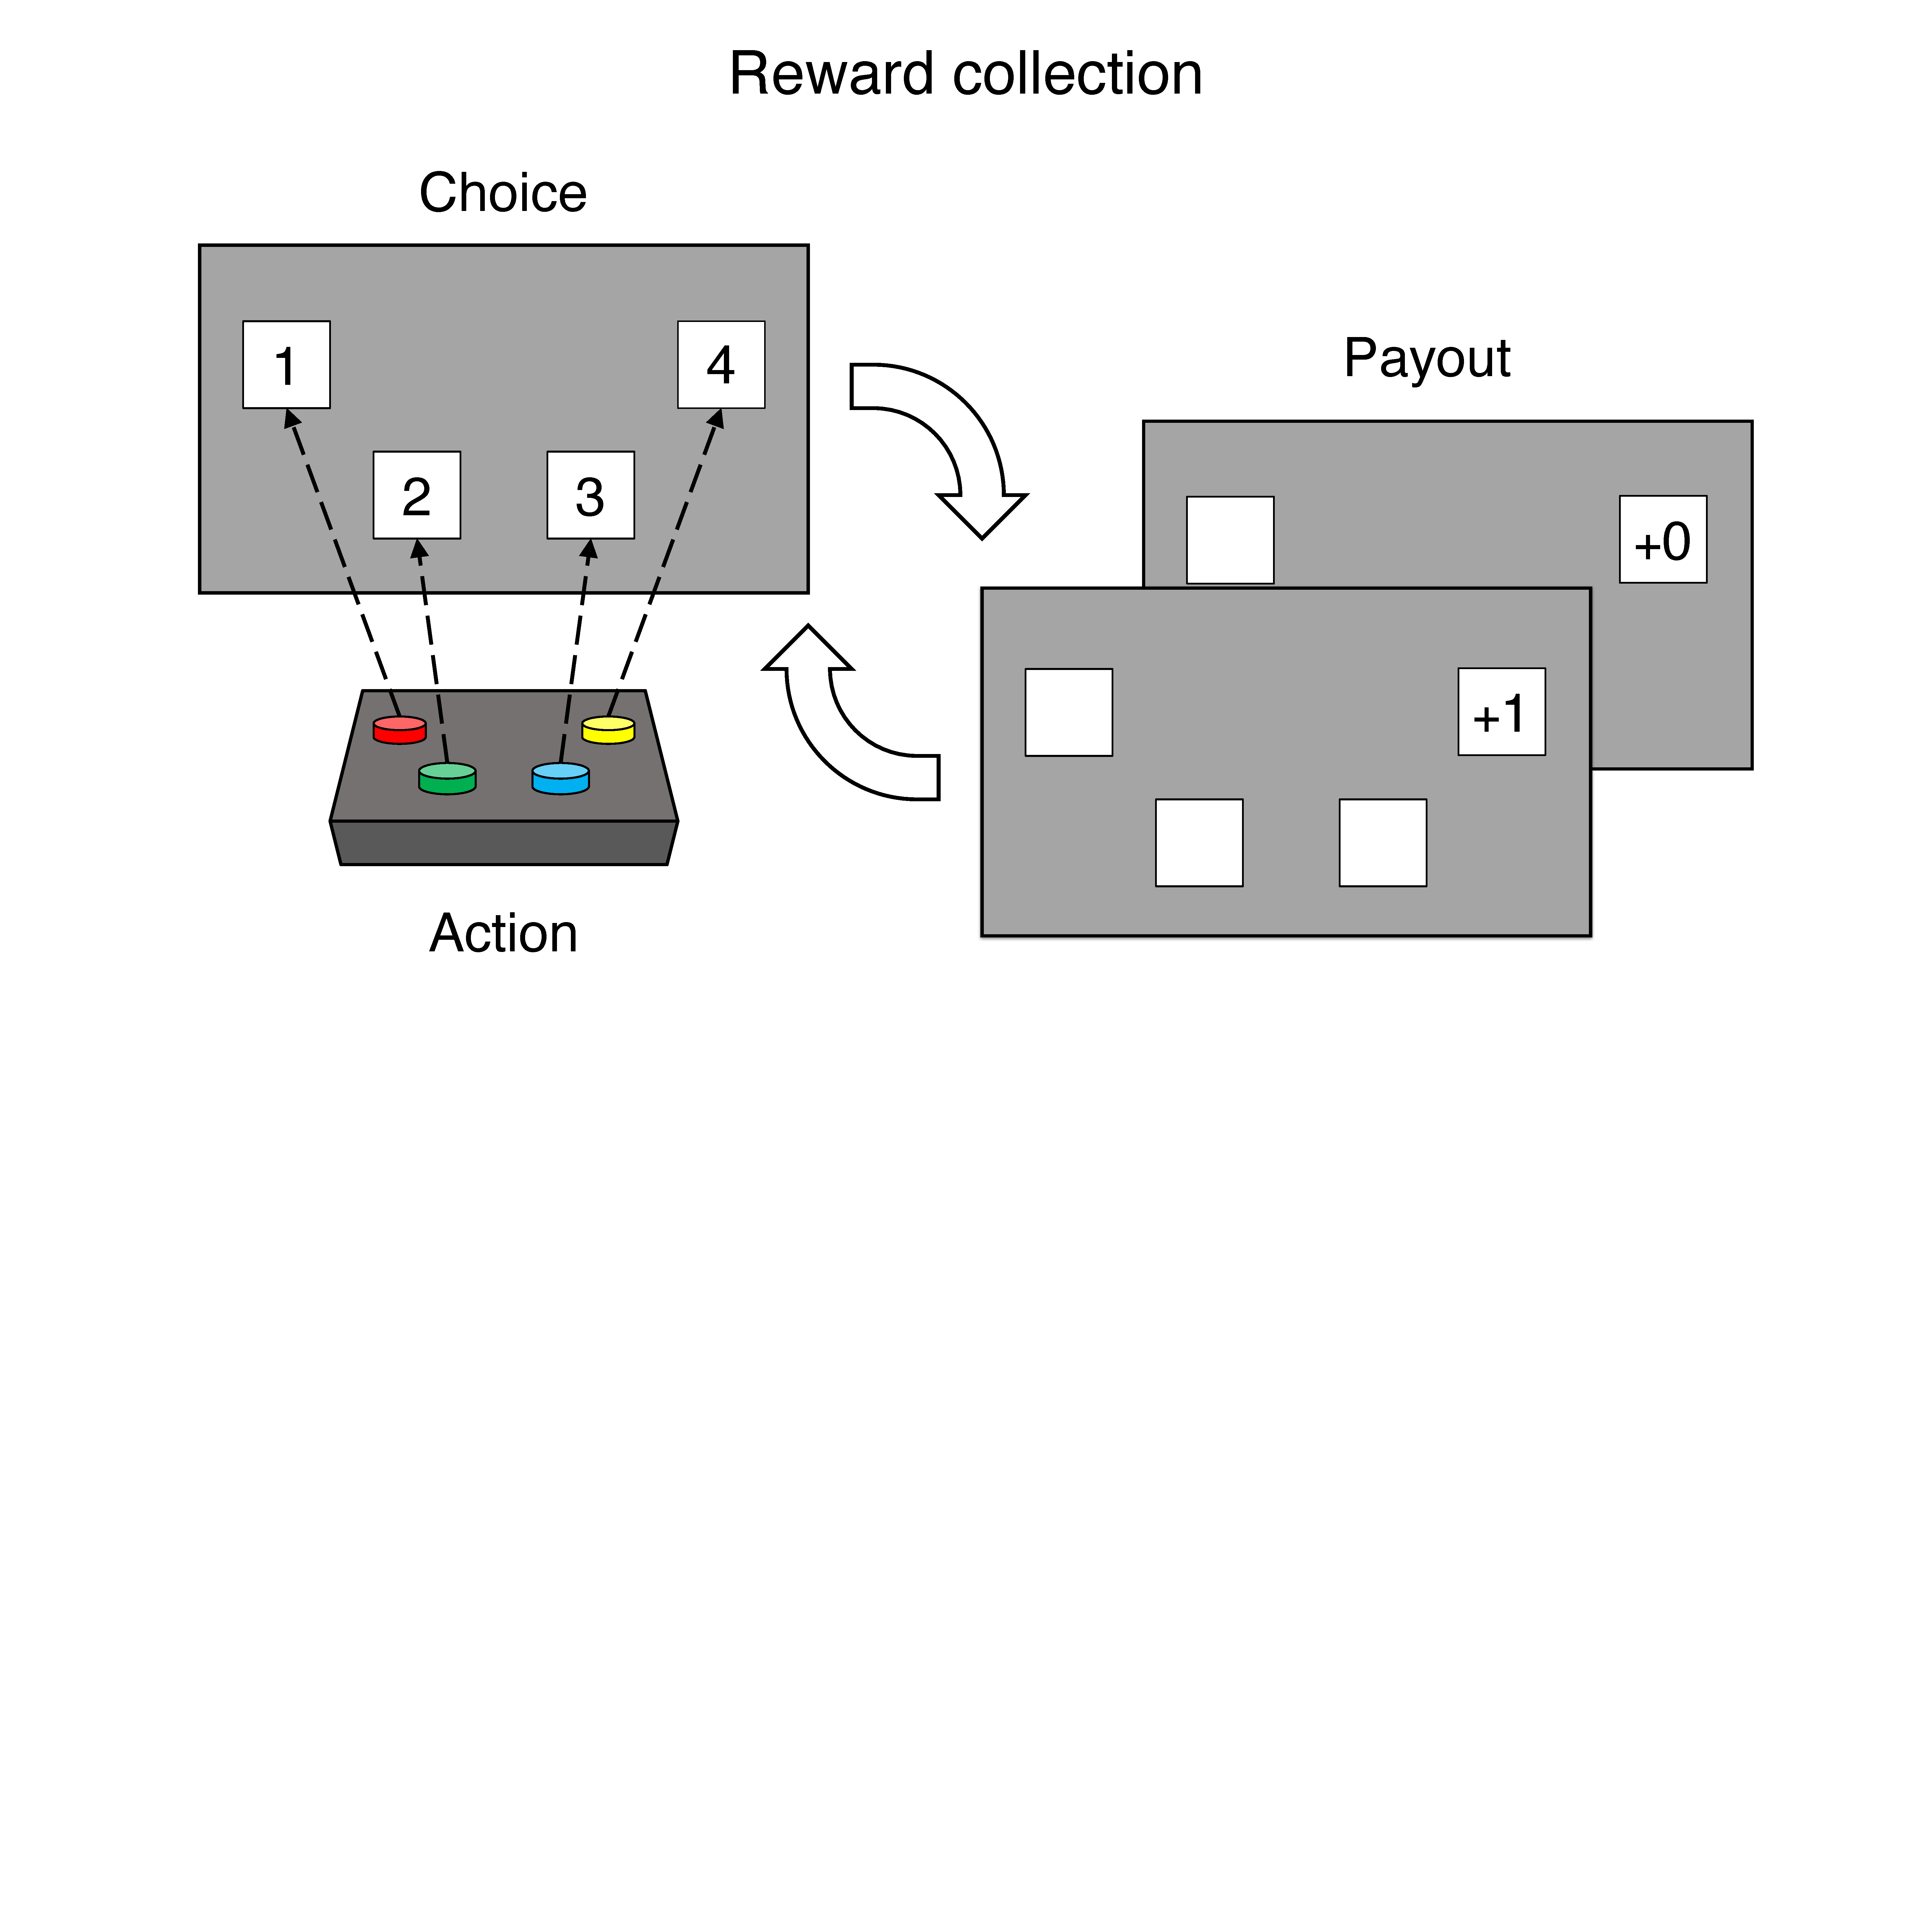
\includegraphics[width=.55\linewidth]{img/task_outline2.pdf} 
	\caption{A 4 choice reward collection task. The reward is numerical value, here a 1 or 0. A good learner in this task is one who collects the most rewards. The task depicted here matches that in Fig~\ref{fig:payout}b. Every other reward collection task we study has the same basic form, only the number of choices increases and the reward spaces are more complex.}
	\label{fig:task_outline2} 
	\end{fullwidth}
\end{figure}

\begin{figure}
	\begin{fullwidth}
	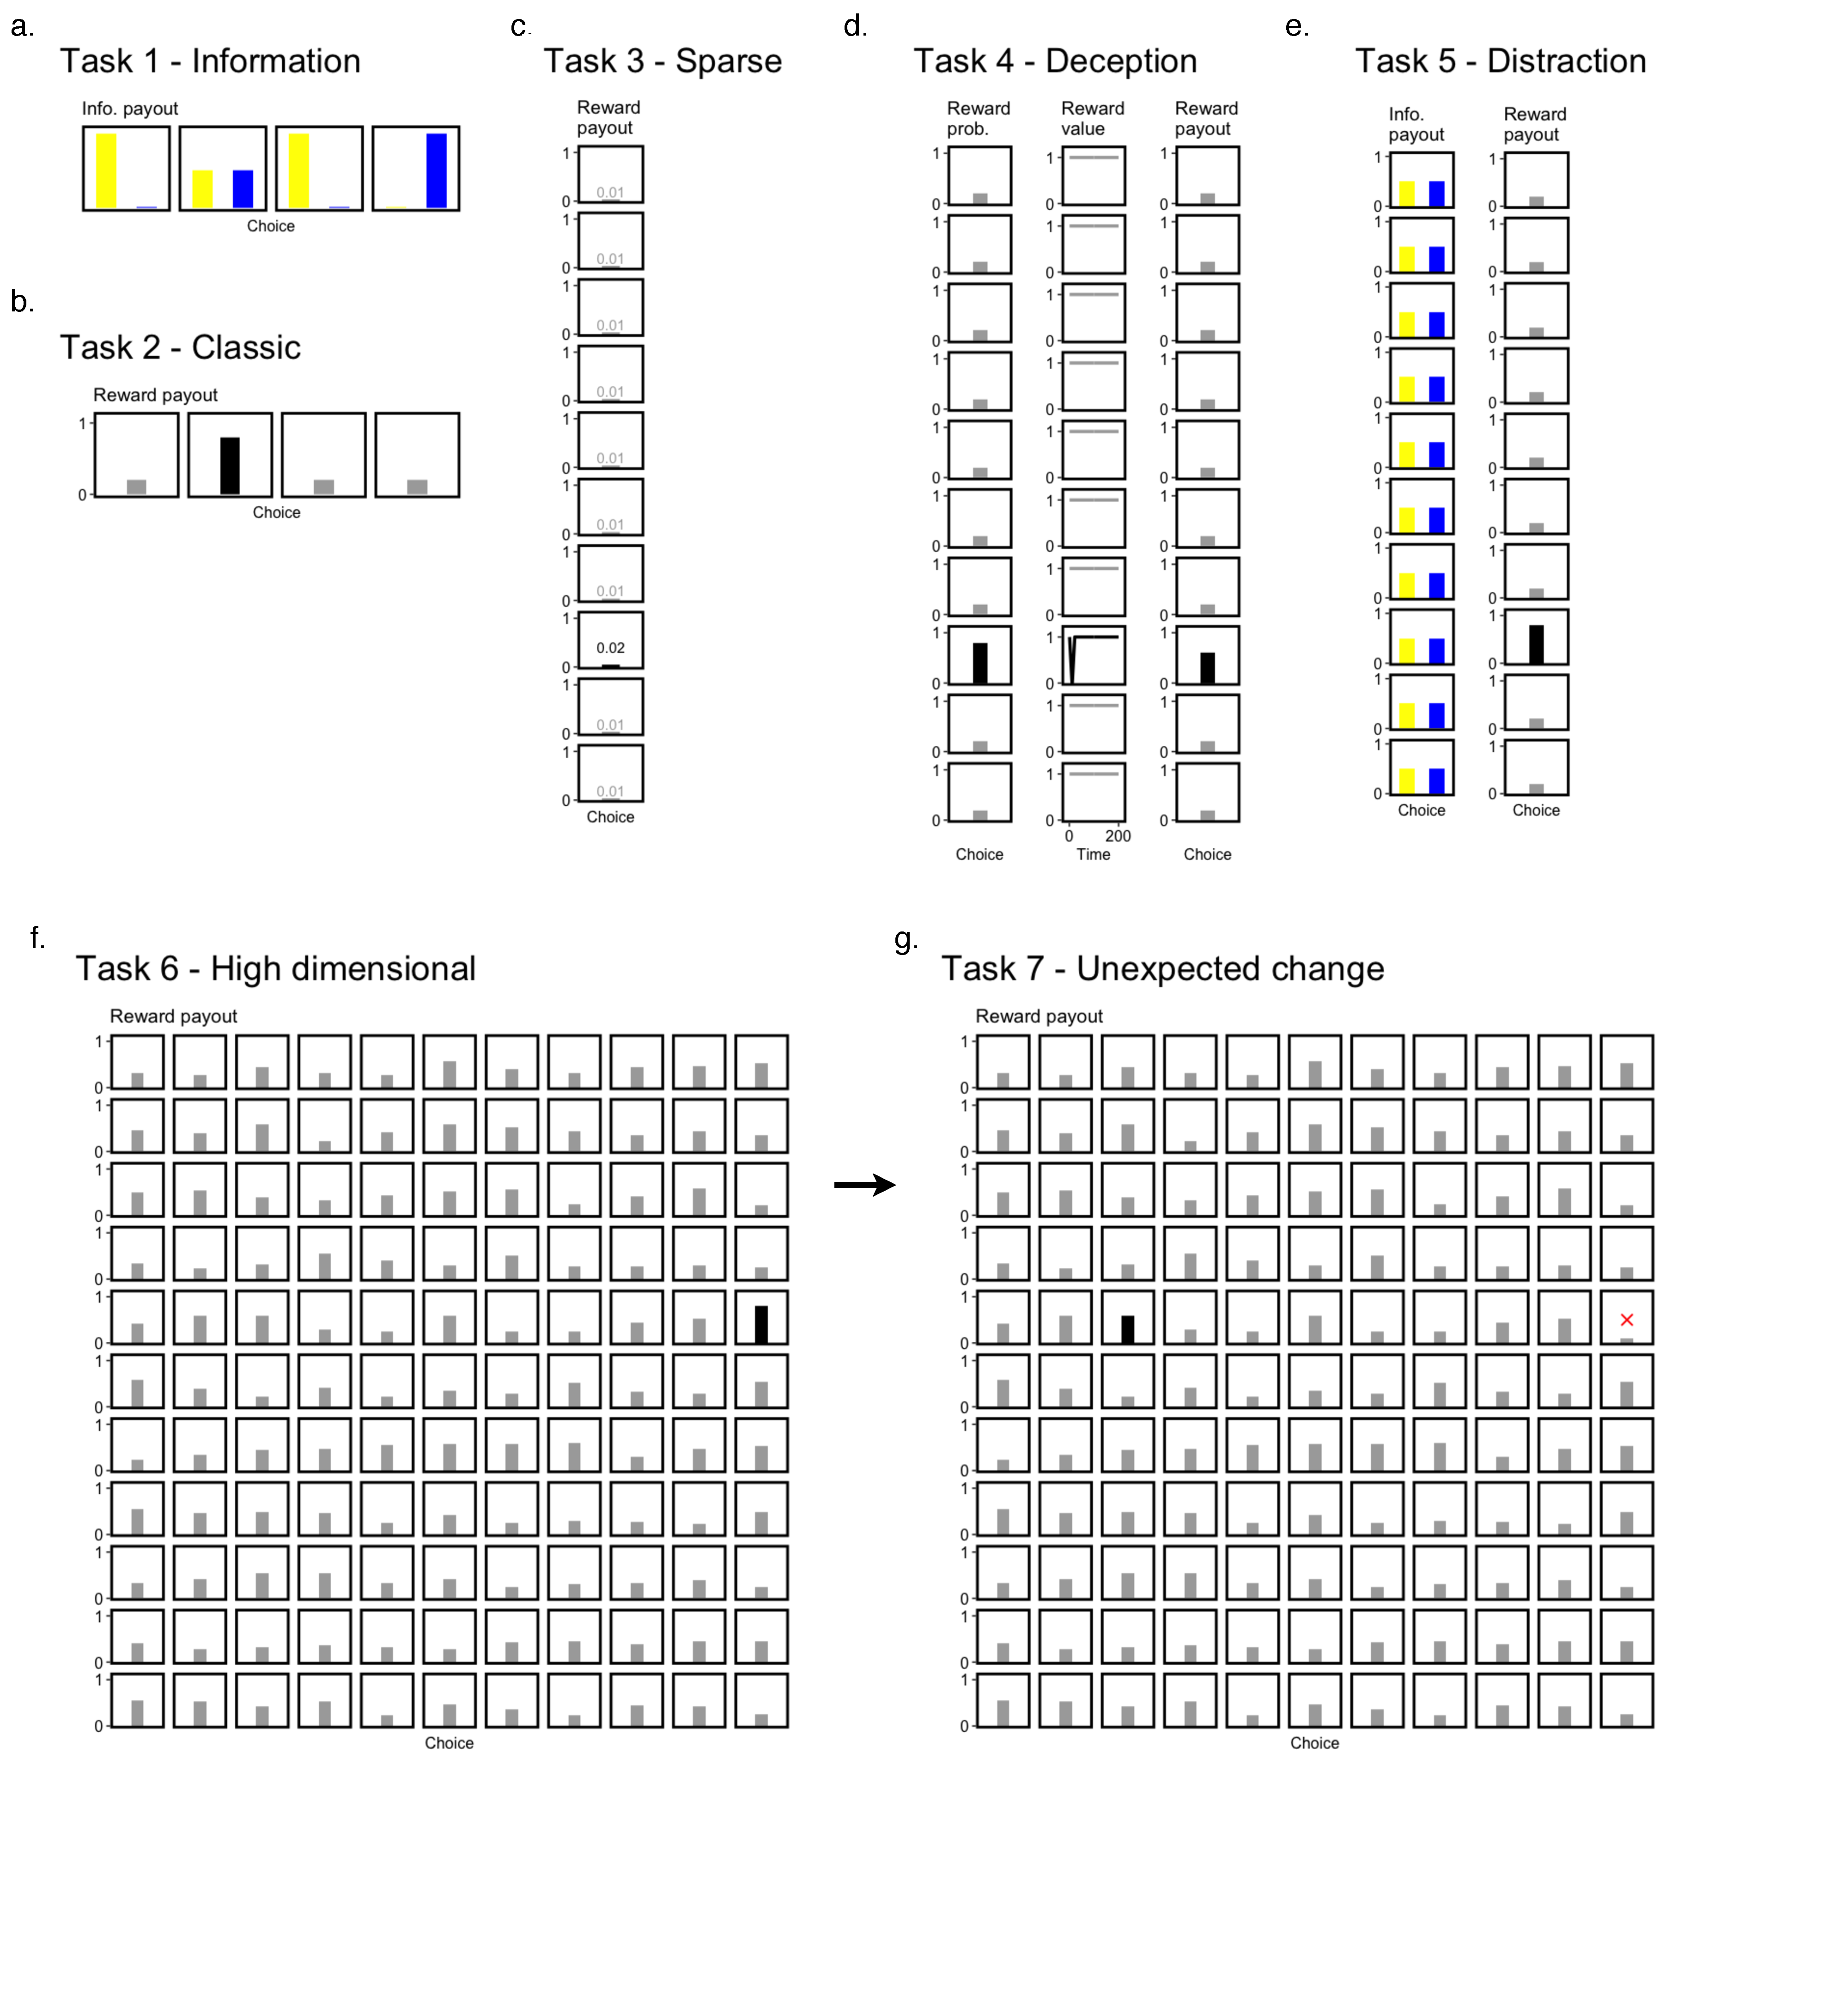
\includegraphics[width=0.9\linewidth]{img/task_payout.pdf} 
	\caption{Payouts for \textit{Tasks 1 - 7}. Payouts can be information, reward, or both. For comments on general task design, see Fig~\ref{fig:task_outline2}.
	\textbf{a.} A classic four-choice design for information collection. A good learner should visit each arm, but quickly discover that only arm two is information bearing.
	\textbf{b.} A classic four-choice design for testing exploration under reward collection. The learner is presented with four choices and it must discover which choice yields the highest average reward. In this task that is Choice 2. 
	\textbf{c.} A ten choice sparse reward task. The learner is presented with four choices and it must discover which choice yields the highest average reward. In this task that is Choice 8 but the very low overall rate of rewards makes this difficult to discover. Solving this task with consistency means consistent exploration. 
	\textbf{d.} A ten choice deceptive reward task. The learner is presented with 10 choices, but the choice which is the best on the long-term (>30 trials) has a lower value in the short term. This value first declines, then rises (see column 2).
	\textbf{e.} A ten choice information distraction task. The learner is presented with both information and rewards. A good learner though will realize the information does not predict reward collection, and so will ignore it.
	\textbf{f.} A 121 choice task with a complex payout structure. This task is thought to be at the limit of human performance. A good learner will eventually discover choice number 57 has the highest payout.
	\textbf{g.} This task is identical to \textit{a.}, except for the high payout choice being changed to be the lowest possible payout. This task tests how well different exploration strategies adjust to simple but sudden change in the environment.
	}
	\label{fig:payout} 
	\end{fullwidth}
\end{figure}

\begin{table}[]
	\caption{Exploration strategies.}
	\label{tab:agents}
	\begin{tabular}{|l|l|l|}
	\hline
	\textbf{Name} & \textbf{Class} & \textbf{Exploration strategy} \\ \hline
	Curiosity & Deterministic & Maximize information value \\ \hline
	Random/Greedy & Random & \begin{tabular}[c]{@{}l@{}}Alternates between random exploration \\ and greedy with probability $\epsilon$.\end{tabular} \\ \hline
	Decay/Greedy & Random & \begin{tabular}[c]{@{}l@{}}The $\epsilon$ parameter \\ decays with a half-life $\tau$\end{tabular} \\ \hline
	Random & Random & Pure random exploration \\ \hline
	Reward & Extrinsic & Softmax sampling of reward value \\ \hline
	Bayesian & Extrinsic + Intrinsic & Sampling of reward value + information value \\ \hline
	Novelty & Extrinsic + Intrinsic & Sampling of reward value + novelty signal \\ \hline
	Entropy & Extrinsic + Intrinsic & Sampling of reward value + action entropy \\ \hline
	Count (EB) & Extrinsic + Intrinsic & Sampling of reward value + visit counts \\ \hline
	Count (UCB) & Extrinsic + Intrinsic & Sampling of reward value + visit counts \\ \hline
	\end{tabular}
\end{table}

\begin{figure}
    \label{fig:summary} 
	\begin{fullwidth}
	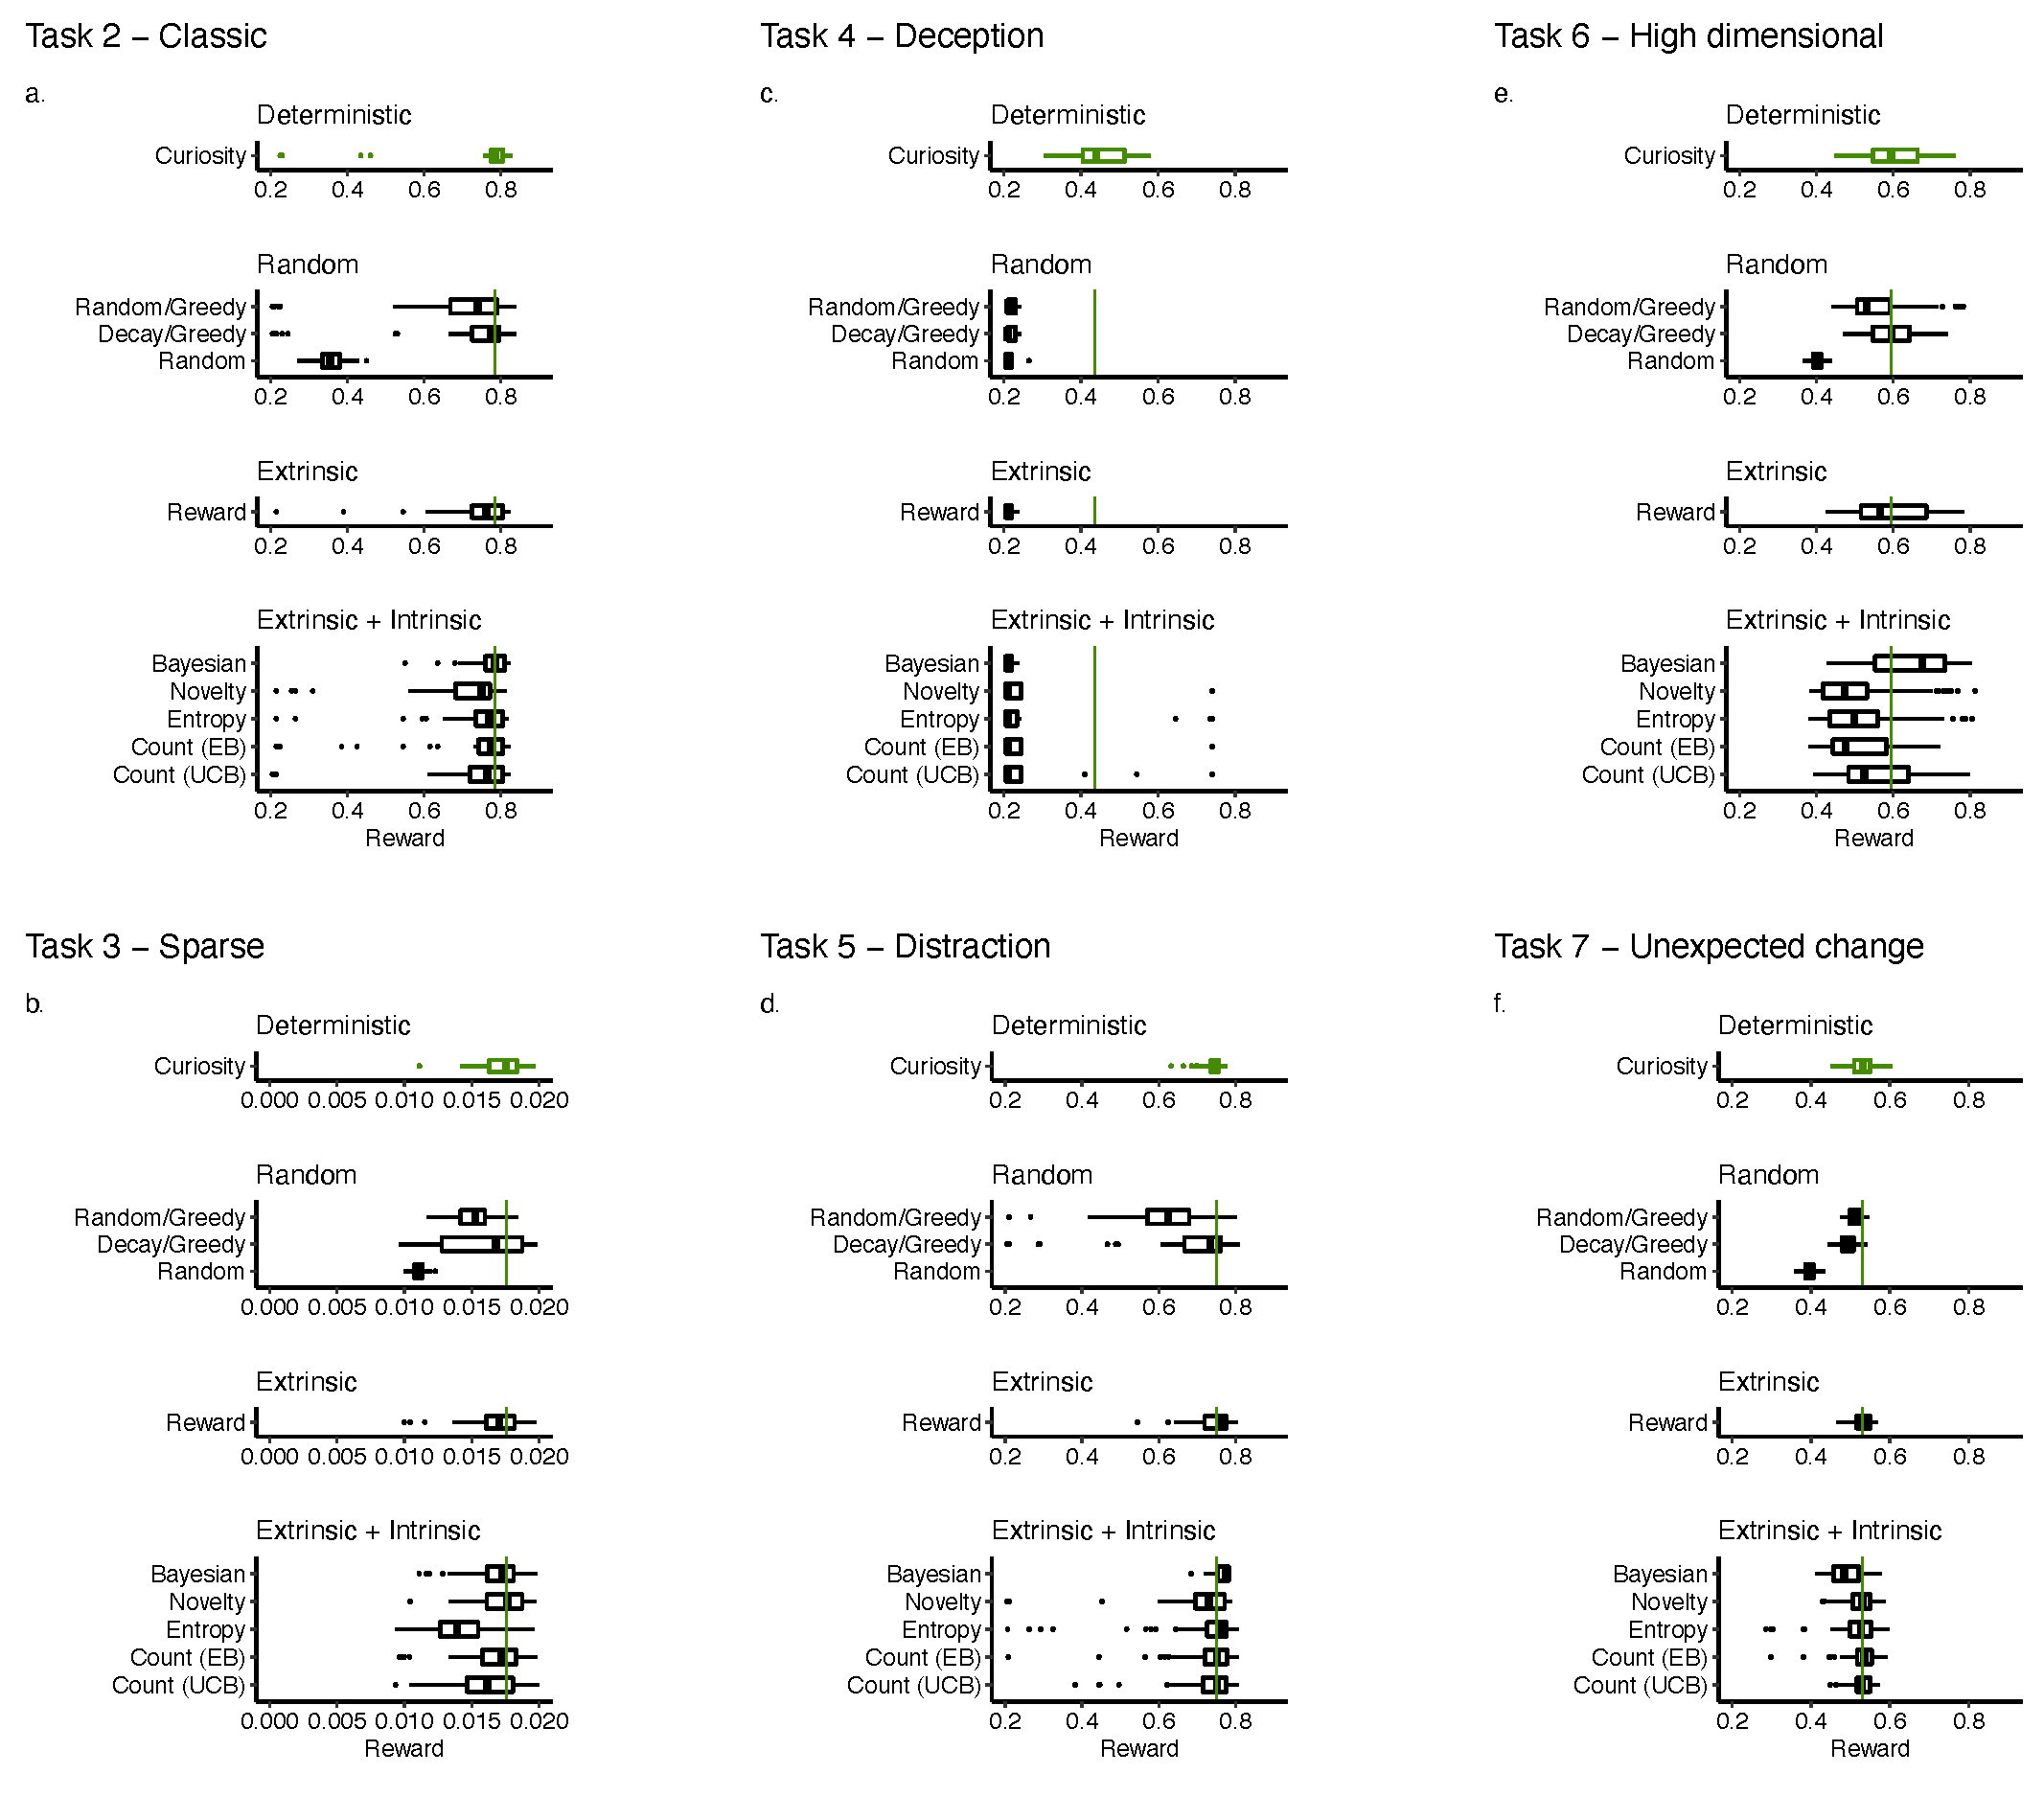
\includegraphics[width=1\linewidth]{img/summary.pdf} 
	\caption{Summary of reward collection (\textit{Tasks 2-7}). The strategies in each panel are grouped according to the class of search they employed (Curiosity. Random, Extrinsic reward or Extrinsic + Intrinsic rewards). 
	\textbf{a.} Results for Task 2, which has four choices and one clear best choice.
	\textbf{b.} Results for Task 3, which has 10 choices and very sparse positive returns.
	\textbf{c.} Results for Task 4, whose best choice is initially ``deceptive'' in that it returns suboptimal reward value over the first 20 trials.
	\textbf{d.} Results for Task 5, which blends the information foraging task 1 with a larger version of Task 2. The yellow/blue stimuli are a max entropy distraction which do not predict the reward payout of each arm.
	\textbf{e.} Results for Task 6, which has 121 choices and a quite heterogeneous set of payouts but still with one best choice.
	\textbf{f.} Results for Task 7, which is identical to Task 6 except the best choice was changed to be the worst. The learners from Task 6 were trained on this Task beginning with the learned values from their prior experience -- a test of robustness to sudden change in the environment. 
	\textit{Note}: To accommodate the fact that different tasks were run different numbers of trials, we normalized total reward by trial number. This lets us plot reward collection results for all tasks on the same scale.
  	}
	
	\figsupp{Summary of regret (\textit{Tasks 2-7})}{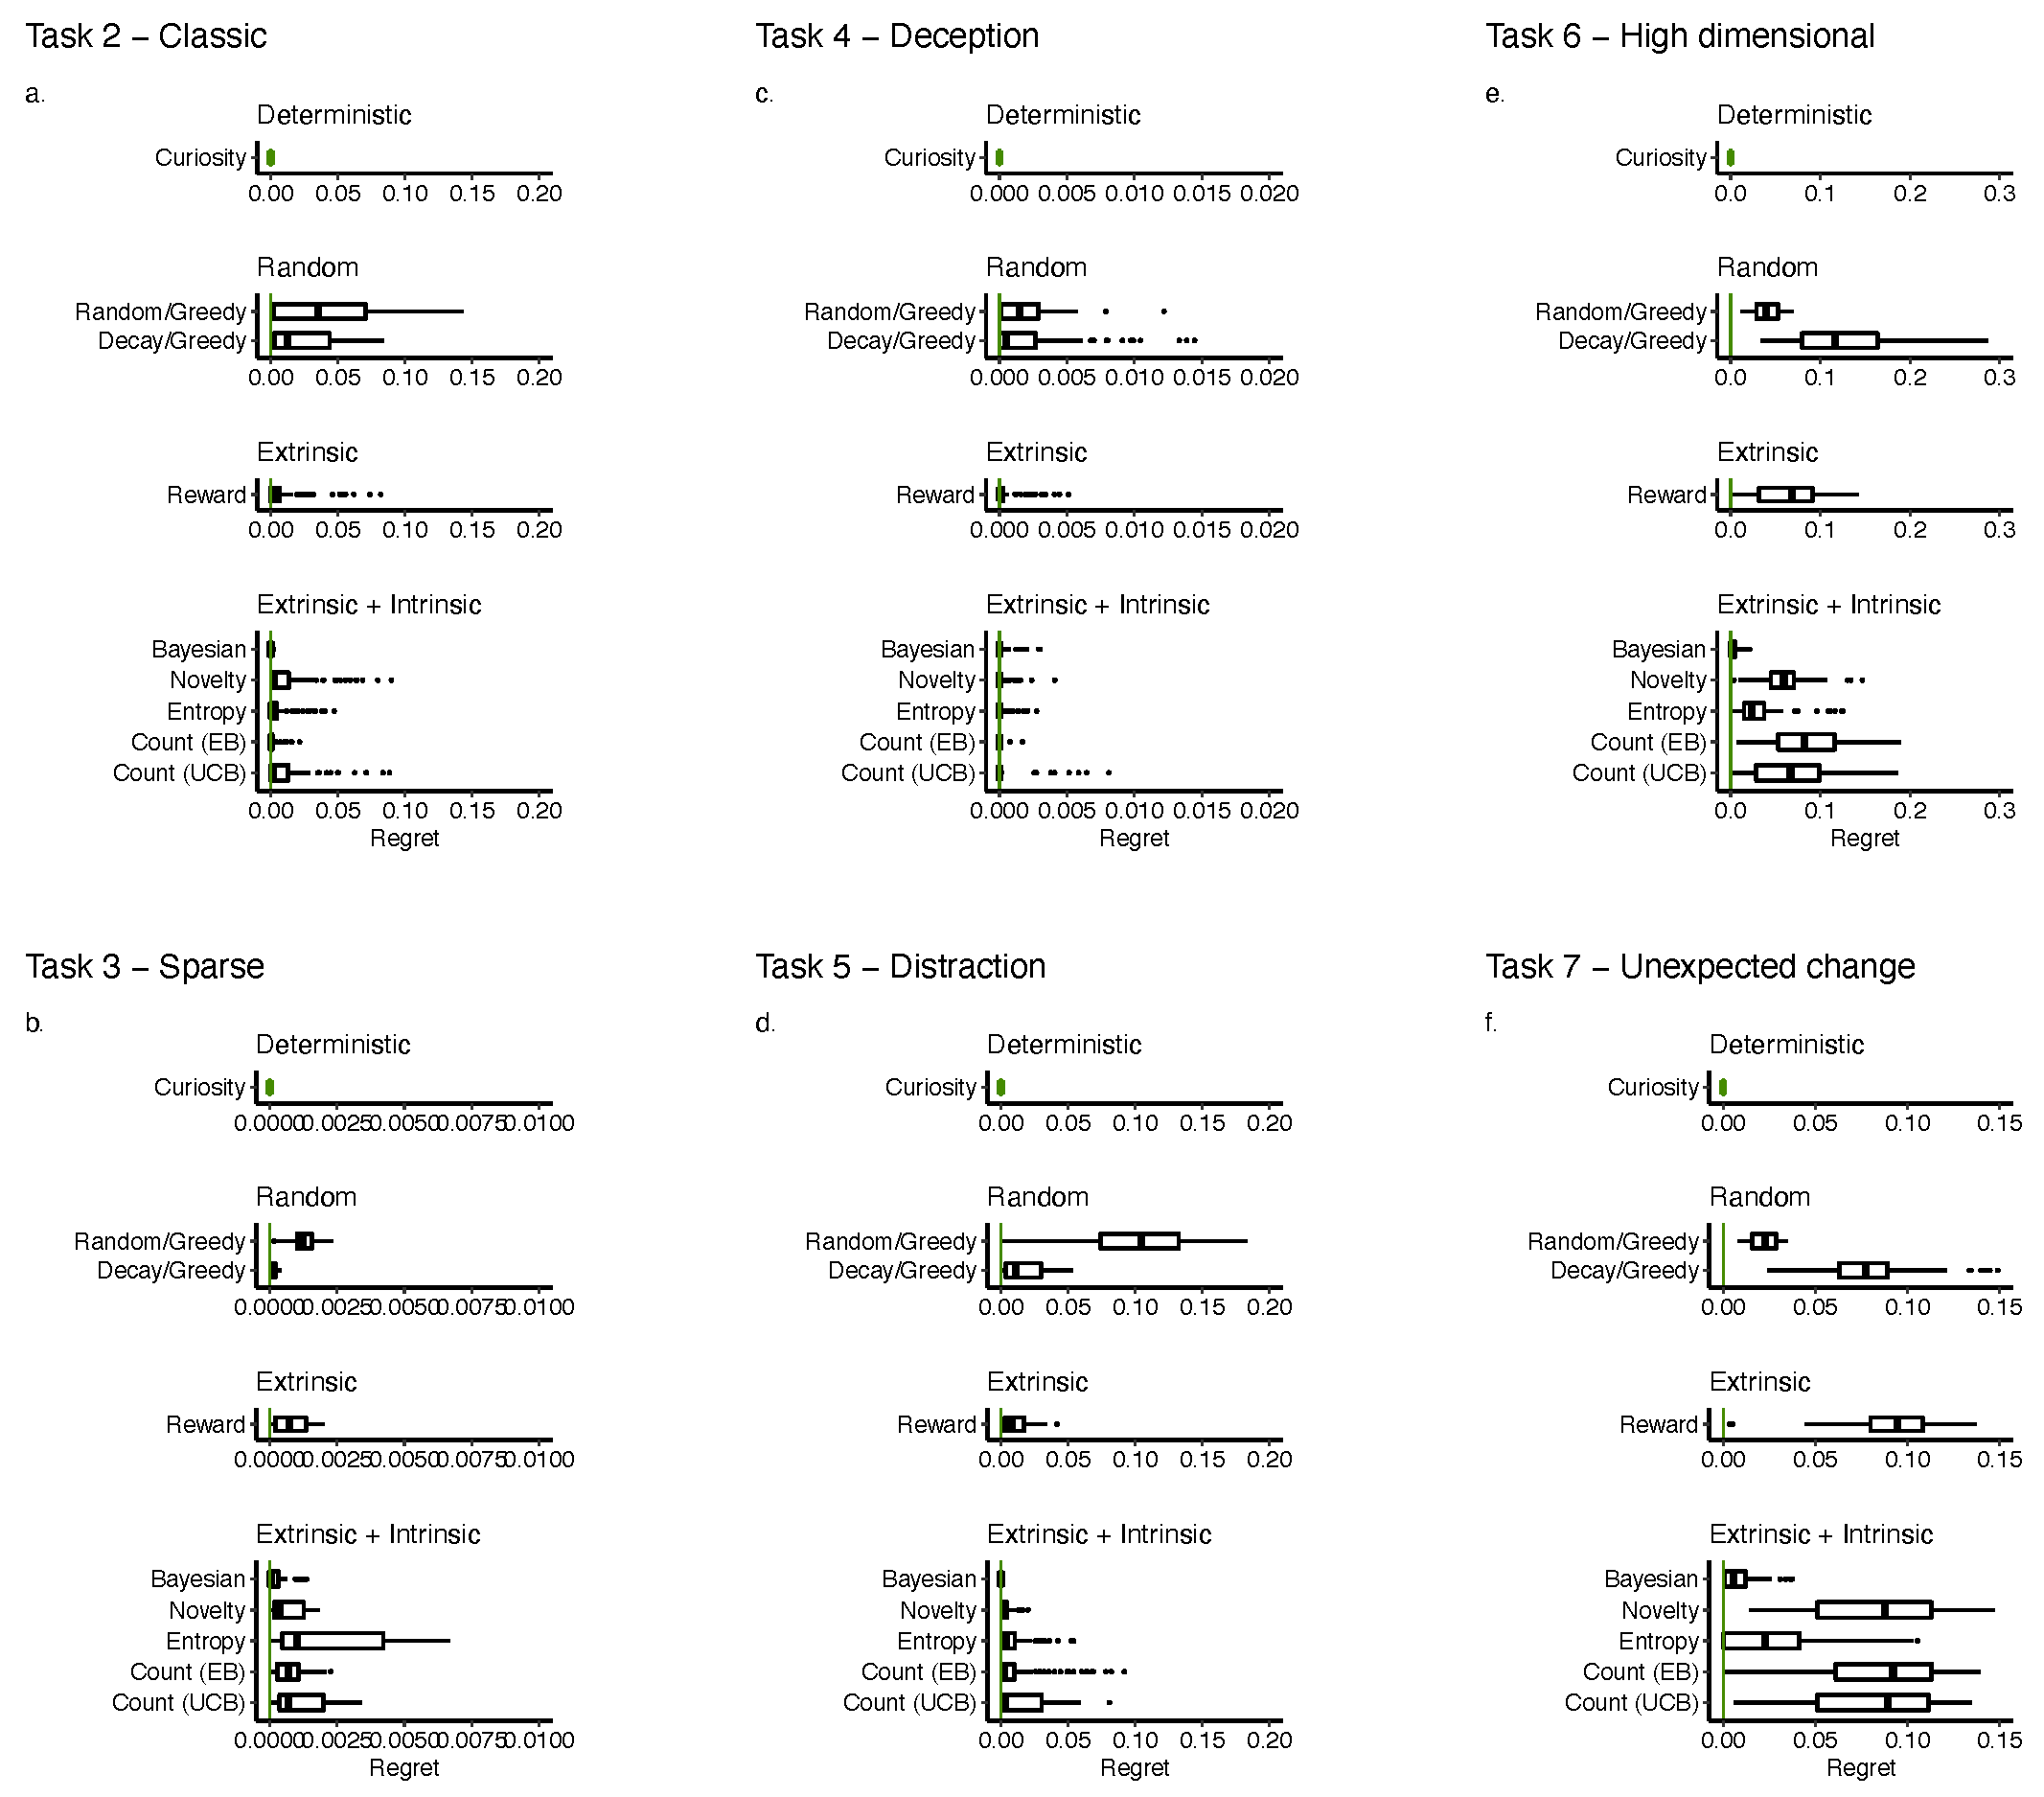
\includegraphics[width=1\linewidth]{img/supp_regret.pdf}}
	\figsupp{Summary of information value (\textit{Tasks 2-7})}{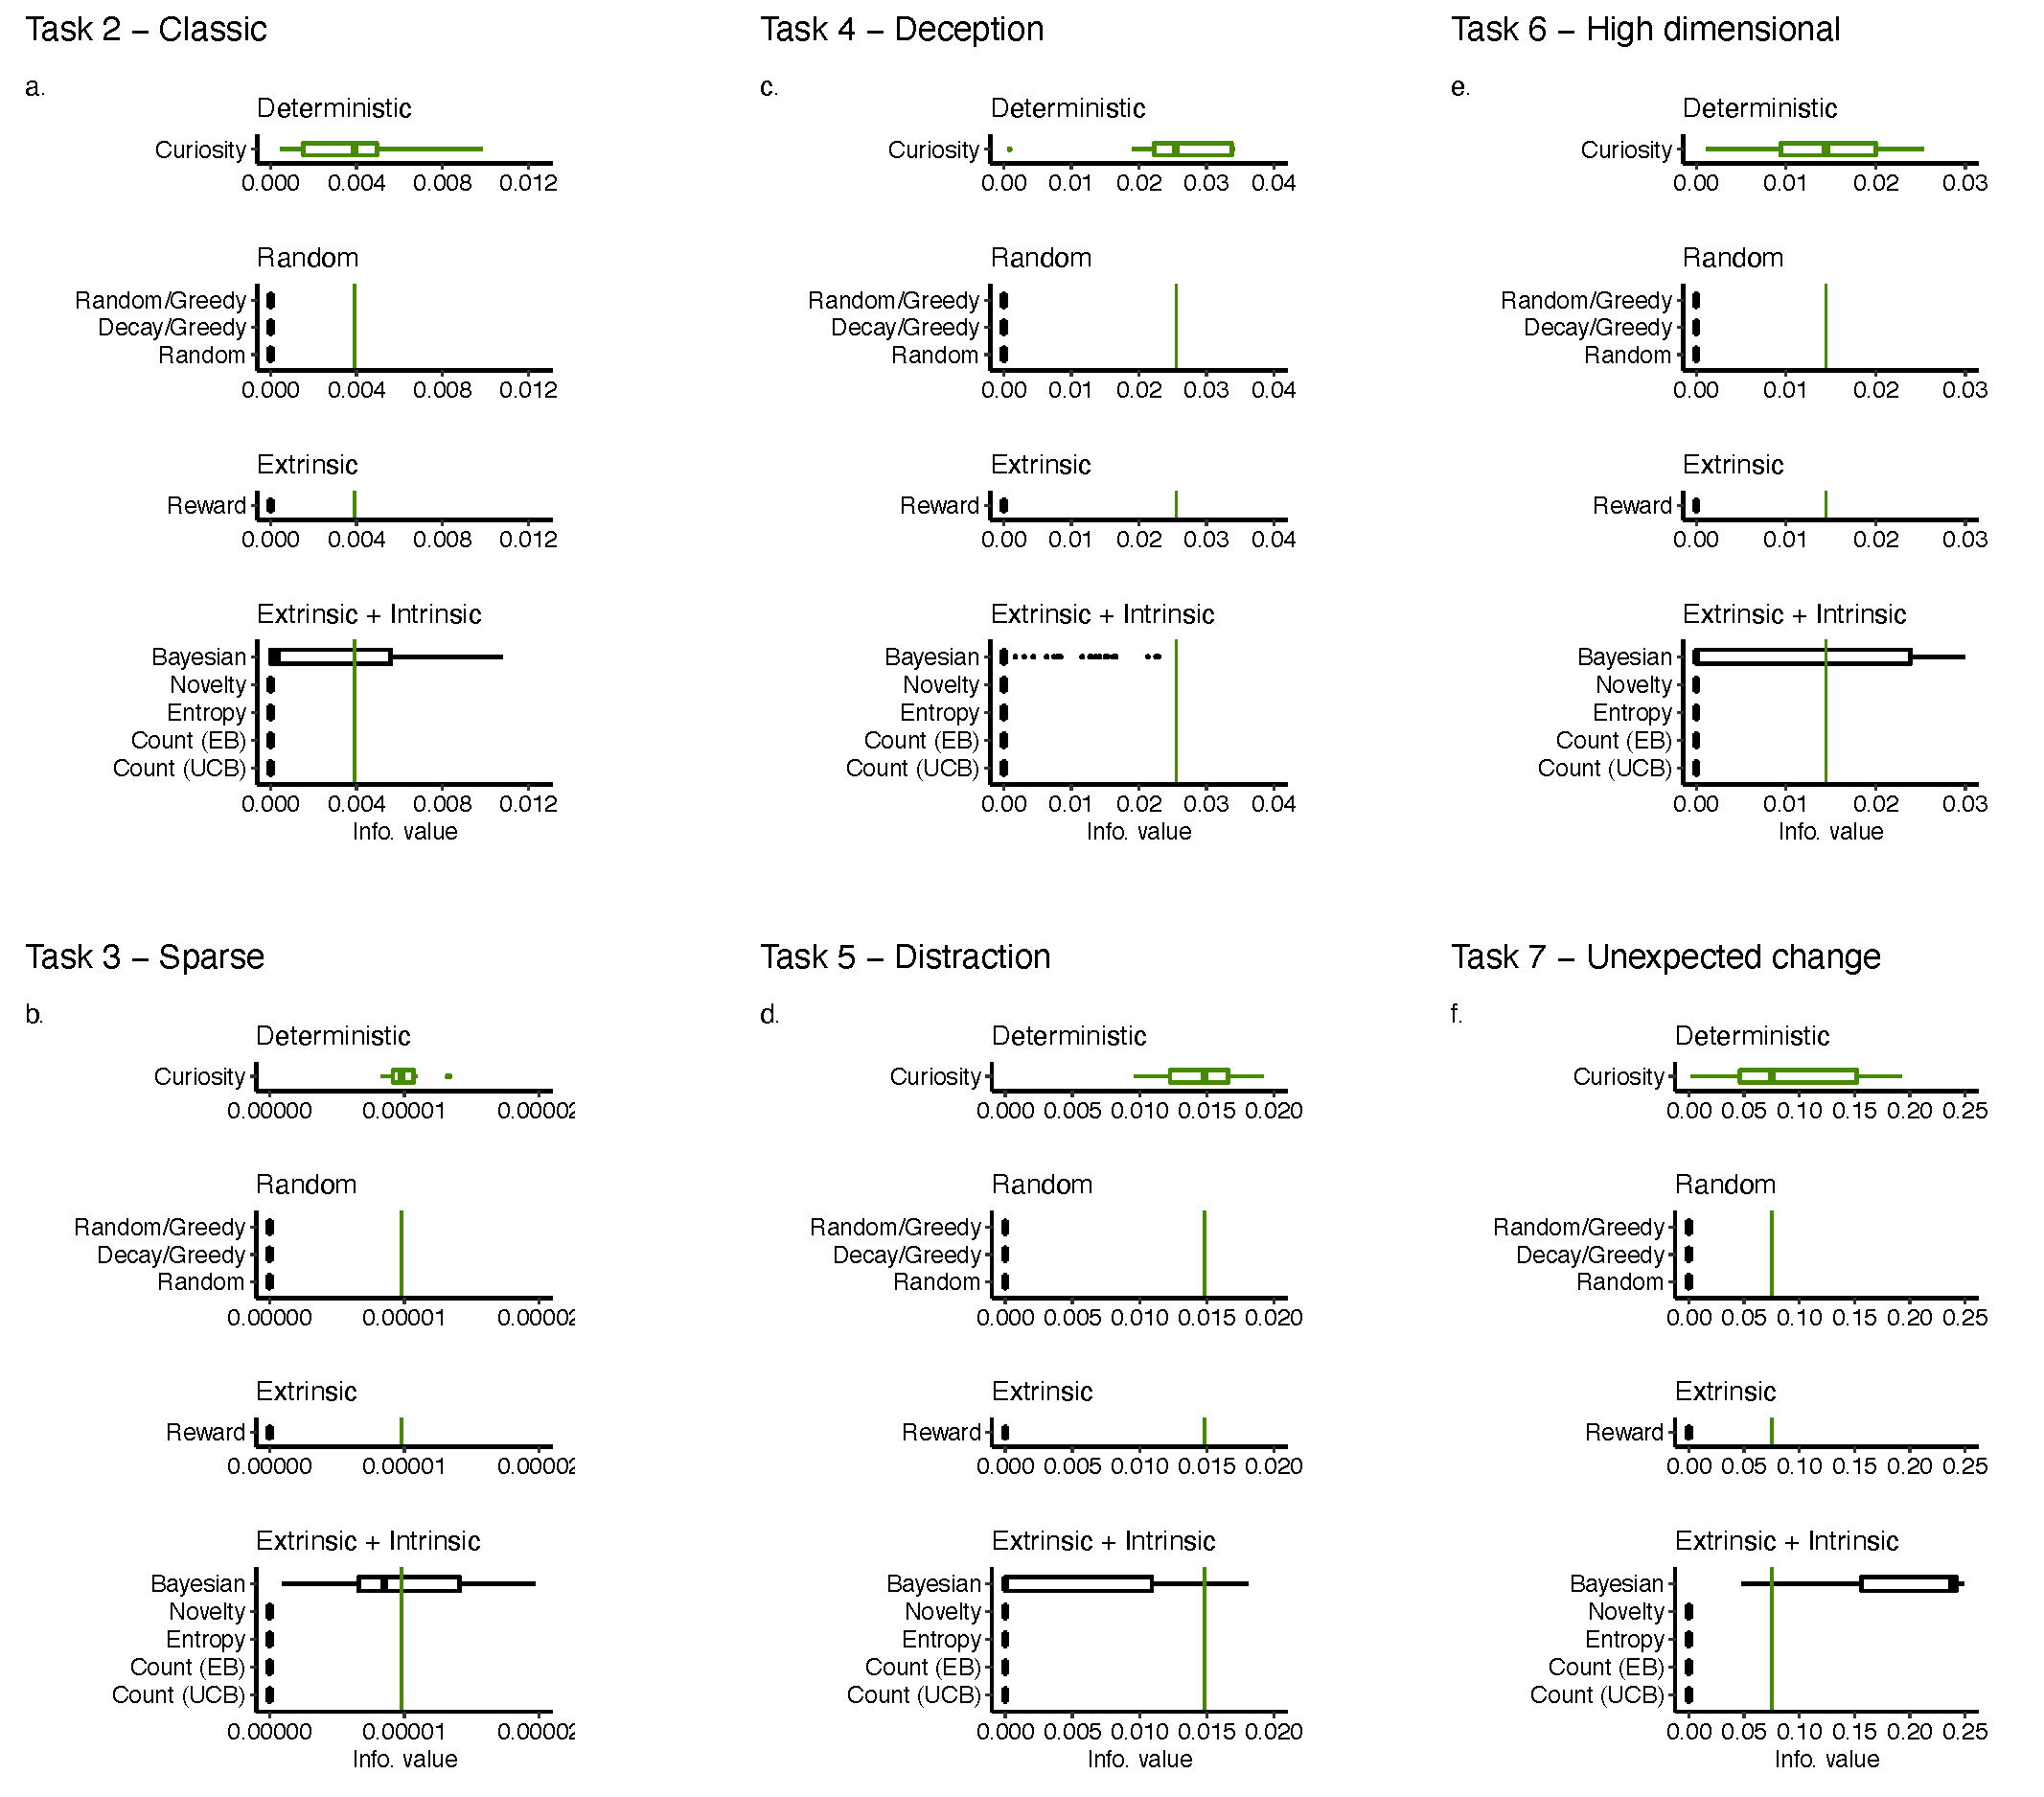
\includegraphics[width=1\linewidth]{img/supp_info.pdf}}
	\figsupp{Examples of exploration (Task 1). Here we simulated different sets of hyper-parameters on the same task and random seed. We view each parameter set as a unique ``animal'' \citep{Prescott2006}. So this figure estimates the degree and kind of variability we might expect in a natural experiment. }{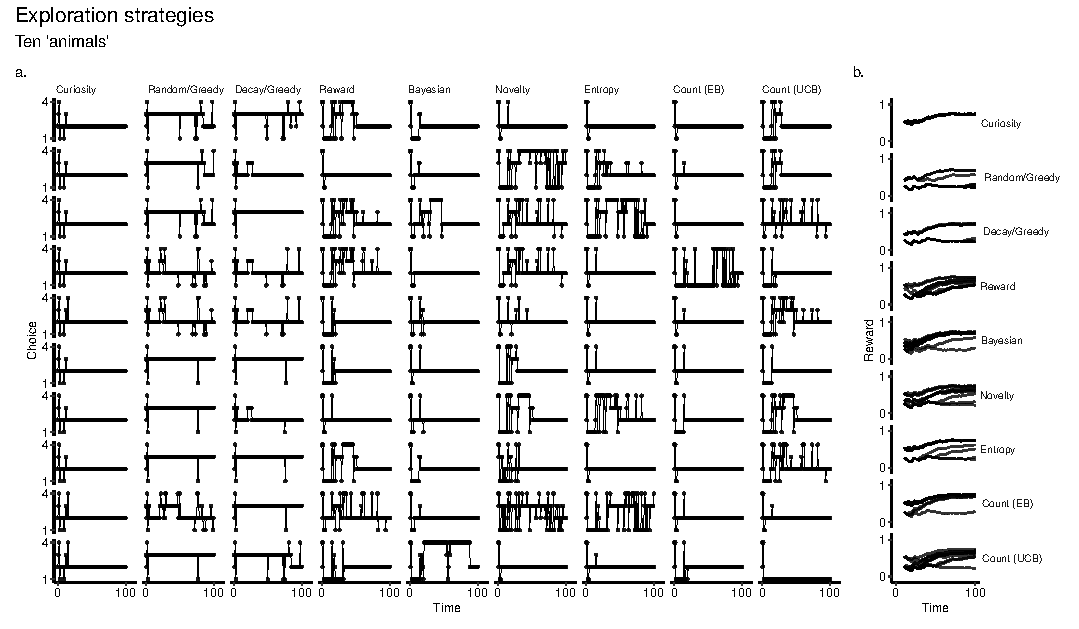
\includegraphics[width=1\linewidth]{img/exploration1.pdf}}
	\end{fullwidth}
\end{figure}

\textit{Task 1.} is an information gathering task, which we discussed already above. \textit{Task 2} was designed to examine reward collection, in probabilistic reward setting very common in the decision making literature \citep{schonberg2007reinforcement,frank2004carrot,cavanagh2014conflict,jahfari2019cross,collins2014opponent,collins2017interactions,glascher2010states}. Rewards were 0 or 1. The best choice had a payout of $p(R=1) = 0.8$. This is a much higher average payout than the others ($p(R=1) = 0.2$). At no point does the task generate symbolic information. See, Fig.~\ref{fig:payout1}\textbf{b}. 

The results for Task 1 were discussed above. As for Task 2, we expected all the exploration strategies to succeed. While this was indeed the case, our deterministic curiosity was the top-performer in terms of median rewards collected, though by a small margin (Fig~\ref{fig:summary}\textbf{a}).

\textit{Task 3.} was designed with very sparse rewards \citep{Mniha,Silver2016b,Silver2018} and there were 10 choices, making this a more difficult task (Fig.~\ref{fig:payout1}\textbf{c}). Sparse rewards are a common problem in the natural world, where an animal may have to travel and search between each meal This is a difficult but not impossible task for vertebrates \citep{anderson1984optimal} and invertebrates \citep{westphal2006foraging}. That being said, most reinforcement learning algorithms will struggle in this setting because the thing they need to learn, that is rewards, are often absent. In this task we saw quite a bit more variation in performance, with the novelty-bonus strategy taking the top slot (this is the only time it does so).

\textit{Task 4.} was designed with deceptive rewards. By deceptive we mean that the best long-term option presents itself initially with a decreasing reward value (Fig.~\ref{fig:payout1}\textbf{d}). Such small deceptions abound in many natural contexts where one must often make short-term sacrifices \citep{internicola2012bumble}. It is well known that classic reinforcement learning will often struggle in this kind of task \citep{Lehman2011a,Sutton2018}. Here our deterministic curiosity is the only strategy that reaches above chance performance. Median performance of all other strategies are similar to the random control (Fig~\ref{fig:summary}\textbf{c}). 

\textit{Task 5} was designed to fool curiosity, our algorithm, by presenting information that was utterly irrelevant to reward collection, but had very high entropy and so ``interesting'' to our algorithm. We fully anticipated that this context would fool just our algorithm, with all other strategies performing well since they are largely agnostic to entropy. However, despite being designed to fail, deterministic curiosity still produced a competitive performance to the other strategies (Fig~\ref{fig:summary}\textbf{d}). 

\textit{Tasks 6-7} were designed as a pair, with both having 121 choices, and a complex payout structure. Tasks of this size are at the limit of human performance \citep{Wu2018}. We first trained all learners on \textit{Task 6}, then tested them in Task 7 which identical to 6, except the best payout arm is reset to be worst (Fig.~\ref{fig:payout1}\textbf{e}-\textbf{f}). In other words Tasks 6 and 7 were joined to measure learning in a high dimensional, but shifting, environments.

In Task 6 deterministic curiosity performed well, securing a second place finish. We note the Bayesian strategy  outperformed our approach. However, under the sudden non-stationarity in reward when switching tasks, the top Bayesian model became the worst on Task 7, and deterministic curiosity took the top spot. Compare Fig.~\ref{fig:summary}\textbf{e} to \textbf{f}. This is the robustness that we'd expect for any curiosity algorithm, whose main goal is to learn everything unbiased by other objectives. The environment and the objectives do change in real life, and so we must be prepared for this. Note how the other less-biased-toward-reward-value exploration models (count-based, novelty, and entropy models) also saw gains, to a lesser degree.

\subsection{Robustness}
A good choice of boredom $eta$ is critical for our definition of curiosity, and was optimized carefully. We show an example of this importance in Fig.~\ref{fig:boredom2}. On the left hand side we did a random search over 10000 possible parameters to find a value for $\eta$ that produced excellent results. (This was the same kind of search we did to achieve the results shown in Fig. ~\ref{fig:summary}. On the right hand side we choose a value for boredom we knew would lead to a poor relative result. We then ran the 100 different randomly generated simulations which gives us the results seen in Fig.~\ref{fig:boredom2}). 

Carefully optimized boredom converged far more quickly (Fig.~\ref{fig:boredom2}a-b), generating more reward over time (Fig.~\ref{fig:boredom2}c-d), and showed far more in consistency during exploration (Fig.~\ref{fig:boredom2}e-f). 

These experiments in setting $\eta$ are also useful in demonstrating the wide variance in behavior that is possible with a deterministic search. Exploration in these figures is deterministic, as prescribed by Eq.~\ref{eq:meta_greedy}. The environment was stochastic however and so the variations come from the environment changing what is learned, which then changes what the best learner should choose to learn next. 

\begin{figure}
	\begin{fullwidth}
	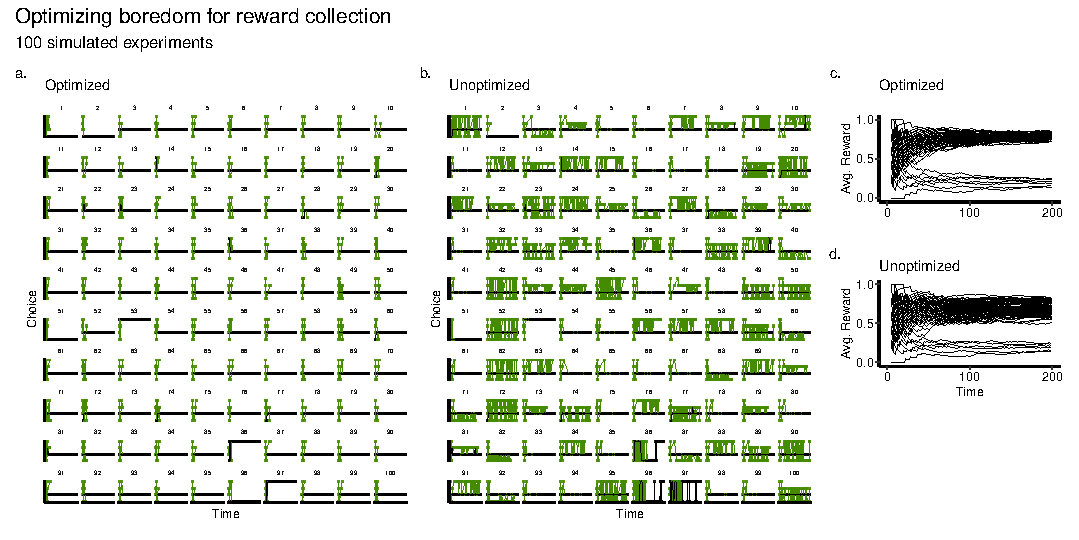
\includegraphics[width=.9\linewidth]{img/boredom2.pdf} 
	\caption{The importance of boredom during reward collection (Task 2). One hundred example experiments, each began with a different random seed. 
	\textbf{a}. Behavioral choices with optimized boredom.
	\textbf{b}. Behavioral choices with unoptimized boredom.
	\textbf{c,d}. Average reward as a function of time for optimized (c) and unoptimized (d) boredom.
	}
	\label{fig:boredom2} 
	\end{fullwidth}
\end{figure}

Unlike idealised simulations, animals cannot pre-optimize their search parameters for every task. We therefore explored reward collection as a function of 1000 randomly chosen model parameters, and reexamined performance on Tasks 1 and 7=6. These were chosen to represent an ``easy'' task, and a ``hard one''. These results are shown in Fig.~\ref{fig:robust}. 

As we observed in our other model comparisons, exploitation by deterministic curiosity produced top-3 performance on both tasks (Fig.~\ref{fig:robust}a-b). Most interesting is the performance for the worst parameters. Here deterministic curiosity was markedly better, with substantially less variability across different parameter schemes. We can explain this in the following way. All the other exploration strategies use parameters to tune the degree of exploration. With deterministic curiosity, however, we tune only when exploration should stop. The degree of exploration, the measure by how close it is to maximum entropy, is fixed by the model itself. It seems that here at least it is far more robust to tune the stopping point, rather than the degree of exploration.

\begin{figure}
	\begin{fullwidth}
	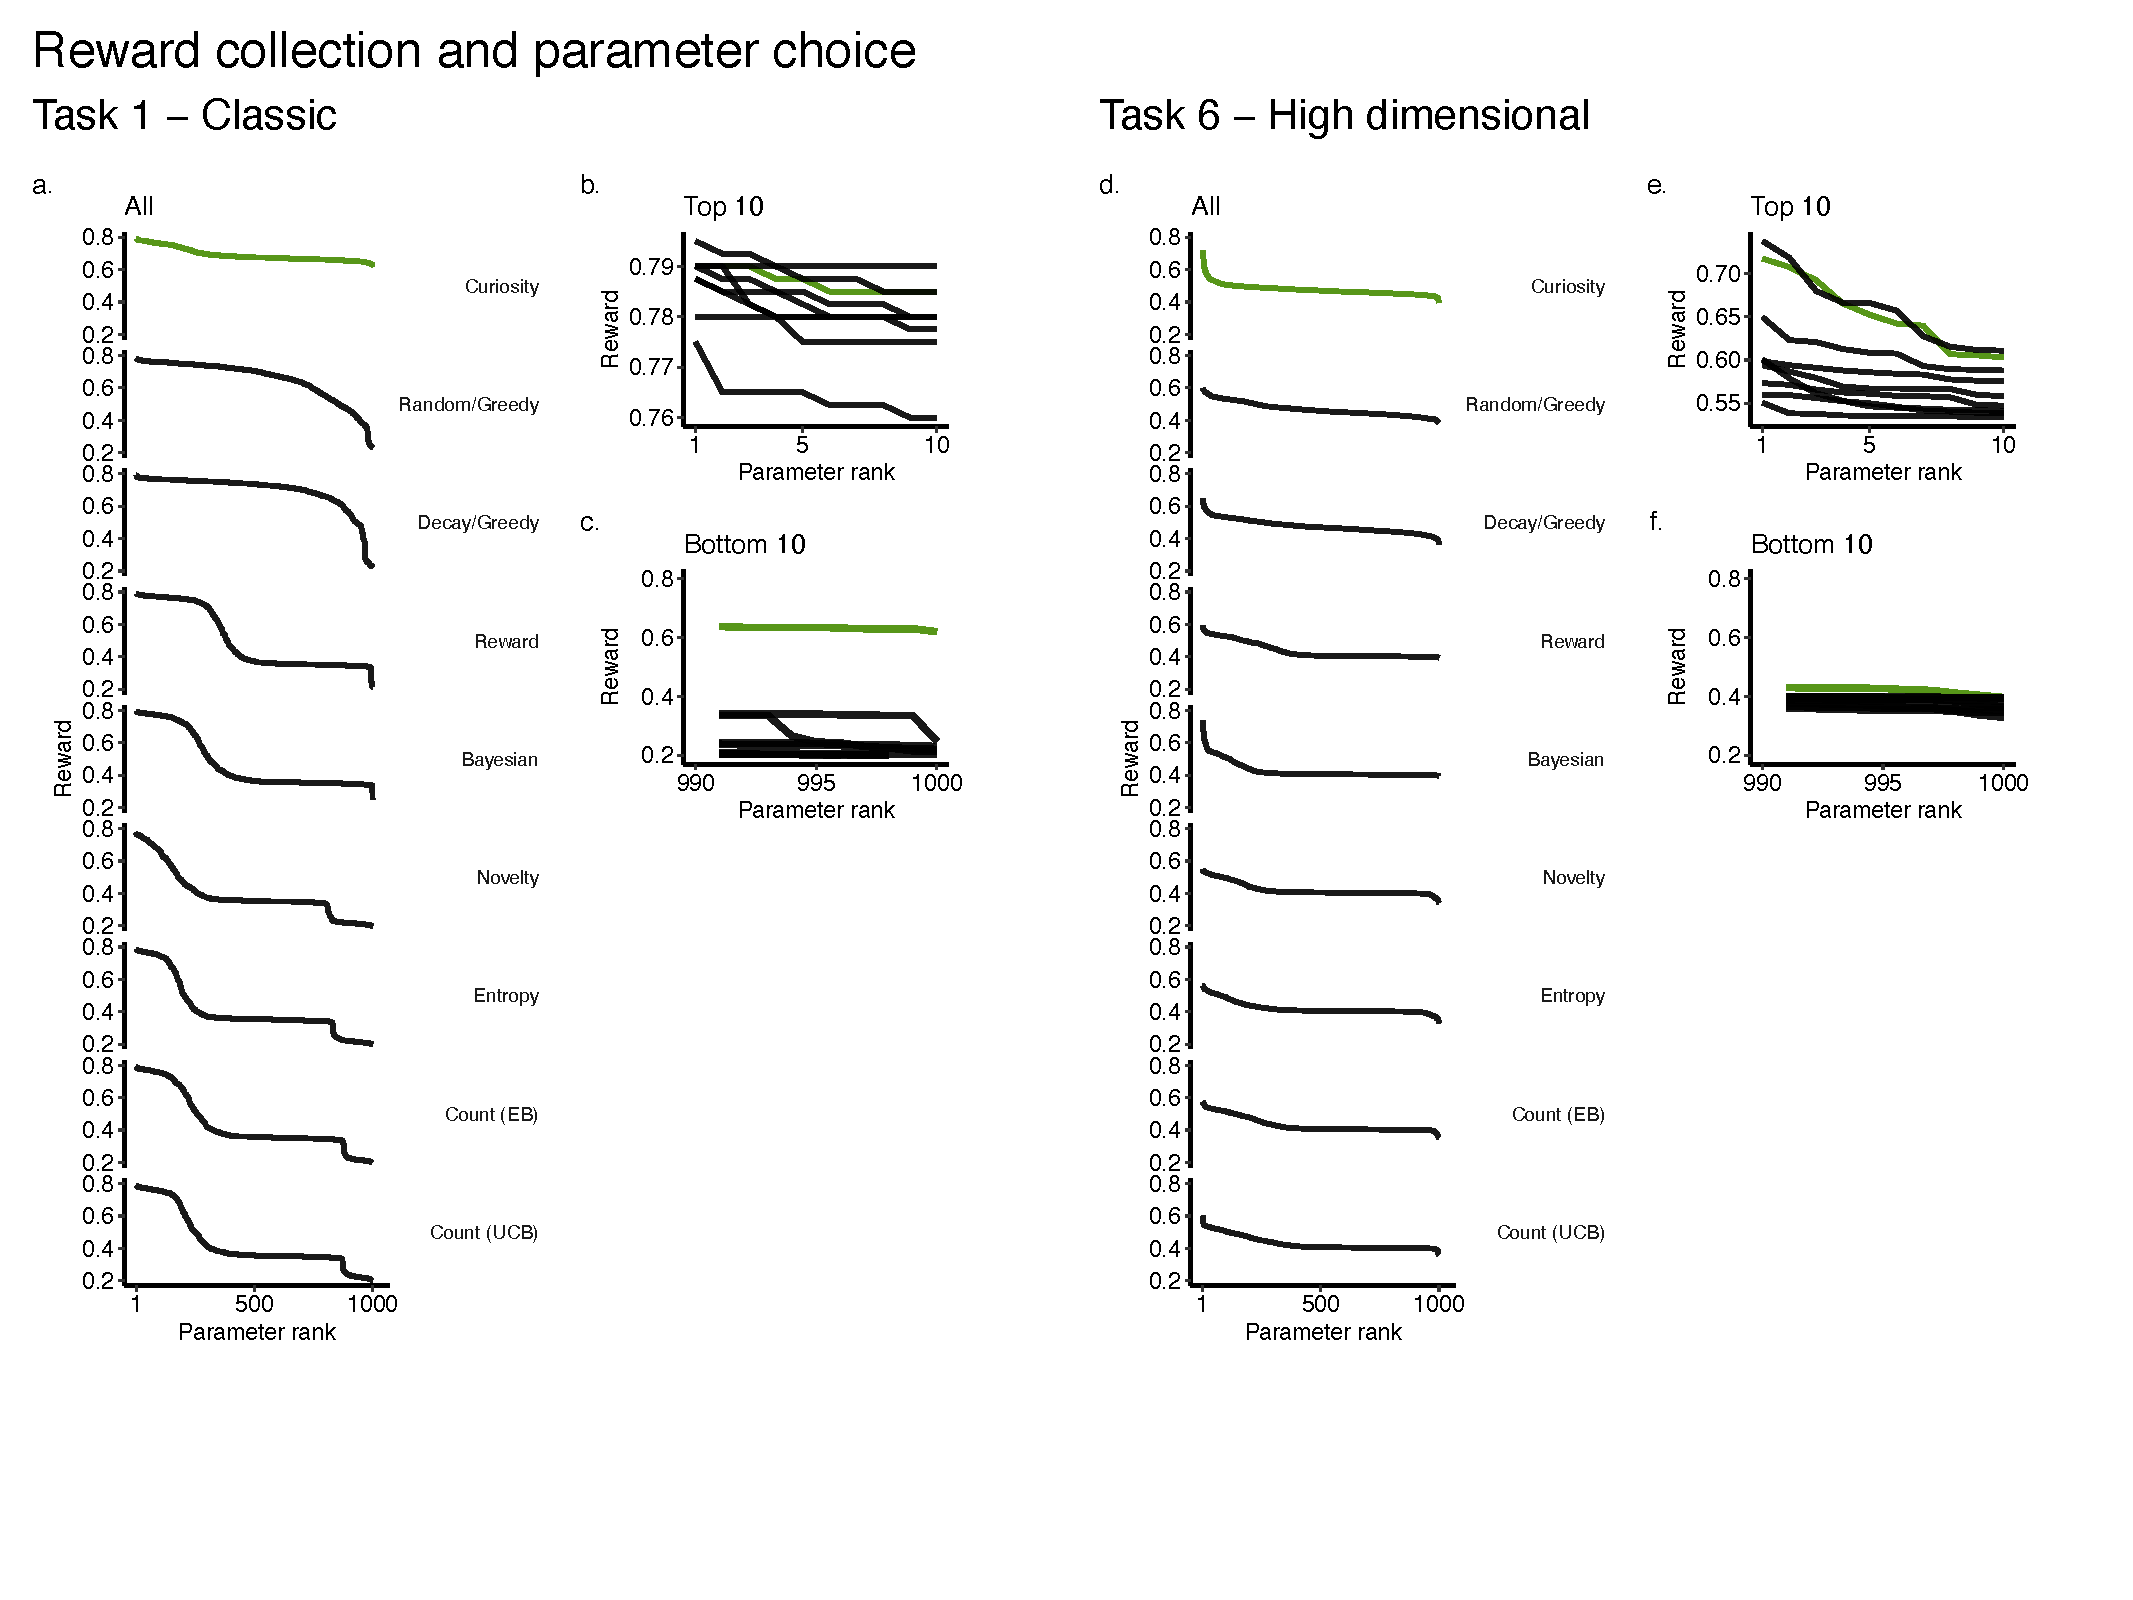
\includegraphics[width=0.8\linewidth]{img/robust.pdf} 
	\caption{Parameter selection and search performance (\textit{Task 2} and \textit{6}). We wanted to evaluate how robust performance was to poor and random hyperparameters. A very robustness exploration algorithm would produce strong performance with both the best parameter choices, and the worst parameter choices.   
	\textbf{a,d} Total reward for 1000 search hyperparameters, for each of strategies we considered.  
	\textbf{b,e} Performance with the top 10 hyperparameters, curiosity (green) compared to all the others.
	\textbf{c.f} Performance with the bottom 10 hyperparameters.
	}
	\figsupp{Adding noise to deterministic curiosity does degrade its performance. In this example control we added two levels of random noise. This only served to increase variability of convergence (a-c) and reduce the total rewards collected (d). Note: decision noise was modelled by sampling a Boltzmann distribution, as described in the \textit{Methods}.
    }{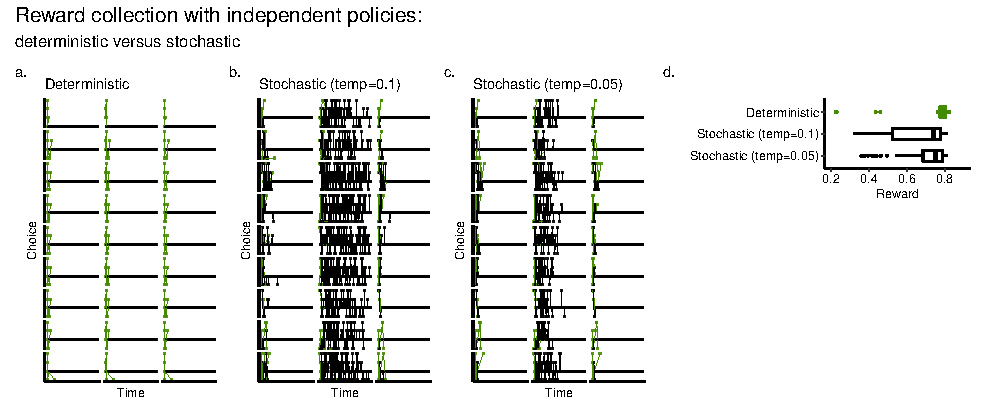
\includegraphics[width=1\linewidth]{img/independent2.pdf}}
    \figsupp{Noise across strategies. Adding noise to degrades performance to nearly the same degree (Task 2).
    }{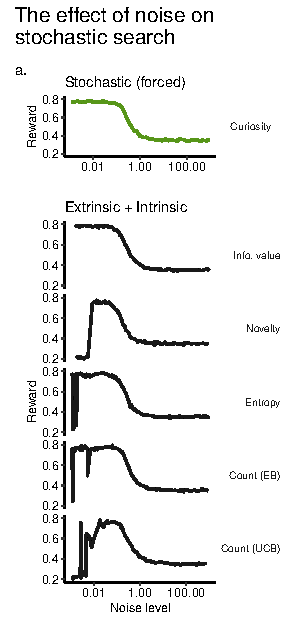
\includegraphics[width=0.3\linewidth]{img/forced2.pdf}}
	\label{fig:robust}
	\end{fullwidth}
\end{figure}
